% Options for packages loaded elsewhere
\PassOptionsToPackage{unicode}{hyperref}
\PassOptionsToPackage{hyphens}{url}
%
\documentclass[
]{article}
\usepackage{amsmath,amssymb}
\usepackage{lmodern}
\usepackage{iftex}
\ifPDFTeX
  \usepackage[T1]{fontenc}
  \usepackage[utf8]{inputenc}
  \usepackage{textcomp} % provide euro and other symbols
\else % if luatex or xetex
  \usepackage{unicode-math}
  \defaultfontfeatures{Scale=MatchLowercase}
  \defaultfontfeatures[\rmfamily]{Ligatures=TeX,Scale=1}
\fi
% Use upquote if available, for straight quotes in verbatim environments
\IfFileExists{upquote.sty}{\usepackage{upquote}}{}
\IfFileExists{microtype.sty}{% use microtype if available
  \usepackage[]{microtype}
  \UseMicrotypeSet[protrusion]{basicmath} % disable protrusion for tt fonts
}{}
\makeatletter
\@ifundefined{KOMAClassName}{% if non-KOMA class
  \IfFileExists{parskip.sty}{%
    \usepackage{parskip}
  }{% else
    \setlength{\parindent}{0pt}
    \setlength{\parskip}{6pt plus 2pt minus 1pt}}
}{% if KOMA class
  \KOMAoptions{parskip=half}}
\makeatother
\usepackage{xcolor}
\usepackage[margin=1in]{geometry}
\usepackage{color}
\usepackage{fancyvrb}
\newcommand{\VerbBar}{|}
\newcommand{\VERB}{\Verb[commandchars=\\\{\}]}
\DefineVerbatimEnvironment{Highlighting}{Verbatim}{commandchars=\\\{\}}
% Add ',fontsize=\small' for more characters per line
\usepackage{framed}
\definecolor{shadecolor}{RGB}{248,248,248}
\newenvironment{Shaded}{\begin{snugshade}}{\end{snugshade}}
\newcommand{\AlertTok}[1]{\textcolor[rgb]{0.94,0.16,0.16}{#1}}
\newcommand{\AnnotationTok}[1]{\textcolor[rgb]{0.56,0.35,0.01}{\textbf{\textit{#1}}}}
\newcommand{\AttributeTok}[1]{\textcolor[rgb]{0.77,0.63,0.00}{#1}}
\newcommand{\BaseNTok}[1]{\textcolor[rgb]{0.00,0.00,0.81}{#1}}
\newcommand{\BuiltInTok}[1]{#1}
\newcommand{\CharTok}[1]{\textcolor[rgb]{0.31,0.60,0.02}{#1}}
\newcommand{\CommentTok}[1]{\textcolor[rgb]{0.56,0.35,0.01}{\textit{#1}}}
\newcommand{\CommentVarTok}[1]{\textcolor[rgb]{0.56,0.35,0.01}{\textbf{\textit{#1}}}}
\newcommand{\ConstantTok}[1]{\textcolor[rgb]{0.00,0.00,0.00}{#1}}
\newcommand{\ControlFlowTok}[1]{\textcolor[rgb]{0.13,0.29,0.53}{\textbf{#1}}}
\newcommand{\DataTypeTok}[1]{\textcolor[rgb]{0.13,0.29,0.53}{#1}}
\newcommand{\DecValTok}[1]{\textcolor[rgb]{0.00,0.00,0.81}{#1}}
\newcommand{\DocumentationTok}[1]{\textcolor[rgb]{0.56,0.35,0.01}{\textbf{\textit{#1}}}}
\newcommand{\ErrorTok}[1]{\textcolor[rgb]{0.64,0.00,0.00}{\textbf{#1}}}
\newcommand{\ExtensionTok}[1]{#1}
\newcommand{\FloatTok}[1]{\textcolor[rgb]{0.00,0.00,0.81}{#1}}
\newcommand{\FunctionTok}[1]{\textcolor[rgb]{0.00,0.00,0.00}{#1}}
\newcommand{\ImportTok}[1]{#1}
\newcommand{\InformationTok}[1]{\textcolor[rgb]{0.56,0.35,0.01}{\textbf{\textit{#1}}}}
\newcommand{\KeywordTok}[1]{\textcolor[rgb]{0.13,0.29,0.53}{\textbf{#1}}}
\newcommand{\NormalTok}[1]{#1}
\newcommand{\OperatorTok}[1]{\textcolor[rgb]{0.81,0.36,0.00}{\textbf{#1}}}
\newcommand{\OtherTok}[1]{\textcolor[rgb]{0.56,0.35,0.01}{#1}}
\newcommand{\PreprocessorTok}[1]{\textcolor[rgb]{0.56,0.35,0.01}{\textit{#1}}}
\newcommand{\RegionMarkerTok}[1]{#1}
\newcommand{\SpecialCharTok}[1]{\textcolor[rgb]{0.00,0.00,0.00}{#1}}
\newcommand{\SpecialStringTok}[1]{\textcolor[rgb]{0.31,0.60,0.02}{#1}}
\newcommand{\StringTok}[1]{\textcolor[rgb]{0.31,0.60,0.02}{#1}}
\newcommand{\VariableTok}[1]{\textcolor[rgb]{0.00,0.00,0.00}{#1}}
\newcommand{\VerbatimStringTok}[1]{\textcolor[rgb]{0.31,0.60,0.02}{#1}}
\newcommand{\WarningTok}[1]{\textcolor[rgb]{0.56,0.35,0.01}{\textbf{\textit{#1}}}}
\usepackage{graphicx}
\makeatletter
\def\maxwidth{\ifdim\Gin@nat@width>\linewidth\linewidth\else\Gin@nat@width\fi}
\def\maxheight{\ifdim\Gin@nat@height>\textheight\textheight\else\Gin@nat@height\fi}
\makeatother
% Scale images if necessary, so that they will not overflow the page
% margins by default, and it is still possible to overwrite the defaults
% using explicit options in \includegraphics[width, height, ...]{}
\setkeys{Gin}{width=\maxwidth,height=\maxheight,keepaspectratio}
% Set default figure placement to htbp
\makeatletter
\def\fps@figure{htbp}
\makeatother
\setlength{\emergencystretch}{3em} % prevent overfull lines
\providecommand{\tightlist}{%
  \setlength{\itemsep}{0pt}\setlength{\parskip}{0pt}}
\setcounter{secnumdepth}{-\maxdimen} % remove section numbering
\ifLuaTeX
  \usepackage{selnolig}  % disable illegal ligatures
\fi
\IfFileExists{bookmark.sty}{\usepackage{bookmark}}{\usepackage{hyperref}}
\IfFileExists{xurl.sty}{\usepackage{xurl}}{} % add URL line breaks if available
\urlstyle{same} % disable monospaced font for URLs
\hypersetup{
  pdftitle={R Notebook},
  hidelinks,
  pdfcreator={LaTeX via pandoc}}

\title{R Notebook}
\author{}
\date{\vspace{-2.5em}}

\begin{document}
\maketitle

\hypertarget{chapter-9}{%
\section{Chapter 9}\label{chapter-9}}

\hypertarget{section}{%
\subsection{9.9}\label{section}}

\begin{enumerate}
\def\labelenumi{\alph{enumi}.}
\tightlist
\item
\end{enumerate}

\begin{Shaded}
\begin{Highlighting}[]
\FunctionTok{summarize\_normal\_normal}\NormalTok{(}\AttributeTok{mean =} \DecValTok{1000}\NormalTok{, }\AttributeTok{sd =} \DecValTok{2000}\NormalTok{, }\AttributeTok{sigma =} \DecValTok{10}\NormalTok{,}
                        \AttributeTok{y\_bar =} \DecValTok{9000}\NormalTok{, }\AttributeTok{n =} \DecValTok{10000}\NormalTok{)}
\end{Highlighting}
\end{Shaded}

\begin{verbatim}
##       model mean mode   var    sd
## 1     prior 1000 1000 4e+06 2e+03
## 2 posterior 9000 9000 1e-02 1e-01
\end{verbatim}

\begin{enumerate}
\def\labelenumi{\alph{enumi}.}
\setcounter{enumi}{1}
\tightlist
\item
\end{enumerate}

\begin{Shaded}
\begin{Highlighting}[]
\FunctionTok{require}\NormalTok{(rstanarm)}
\end{Highlighting}
\end{Shaded}

\begin{verbatim}
## Loading required package: rstanarm
\end{verbatim}

\begin{verbatim}
## Loading required package: Rcpp
\end{verbatim}

\begin{verbatim}
## This is rstanarm version 2.21.3
\end{verbatim}

\begin{verbatim}
## - See https://mc-stan.org/rstanarm/articles/priors for changes to default priors!
\end{verbatim}

\begin{verbatim}
## - Default priors may change, so it's safest to specify priors, even if equivalent to the defaults.
\end{verbatim}

\begin{verbatim}
## - For execution on a local, multicore CPU with excess RAM we recommend calling
\end{verbatim}

\begin{verbatim}
##   options(mc.cores = parallel::detectCores())
\end{verbatim}

\begin{verbatim}
## 
## Attaching package: 'rstanarm'
\end{verbatim}

\begin{verbatim}
## The following object is masked from 'package:rstan':
## 
##     loo
\end{verbatim}

\begin{Shaded}
\begin{Highlighting}[]
\NormalTok{model }\OtherTok{\textless{}{-}} \FunctionTok{stan\_glm}\NormalTok{(}
\NormalTok{  rides }\SpecialCharTok{\textasciitilde{}}\NormalTok{ humidity, }\AttributeTok{data =}\NormalTok{ bikes, }
  \AttributeTok{family =}\NormalTok{ gaussian,}
  \AttributeTok{prior\_PD =} \ConstantTok{TRUE}\NormalTok{,}
  \AttributeTok{prior\_intercept =} \FunctionTok{normal}\NormalTok{(}\DecValTok{1000}\NormalTok{, }\DecValTok{2000}\NormalTok{, }\AttributeTok{autoscale =} \ConstantTok{TRUE}\NormalTok{),}
  \AttributeTok{prior =} \FunctionTok{normal}\NormalTok{(}\DecValTok{0}\NormalTok{, }\DecValTok{10}\NormalTok{, }\AttributeTok{autoscale =} \ConstantTok{TRUE}\NormalTok{), }
  \AttributeTok{prior\_aux =} \FunctionTok{exponential}\NormalTok{(}\DecValTok{1}\NormalTok{, }\AttributeTok{autoscale =} \ConstantTok{TRUE}\NormalTok{),}
  \AttributeTok{chains =} \DecValTok{5}\NormalTok{, }\AttributeTok{iter =} \DecValTok{8000}\NormalTok{, }\AttributeTok{seed =} \DecValTok{84735}\NormalTok{)}
\end{Highlighting}
\end{Shaded}

\begin{verbatim}
## 
## SAMPLING FOR MODEL 'continuous' NOW (CHAIN 1).
## Chain 1: 
## Chain 1: Gradient evaluation took 1.4e-05 seconds
## Chain 1: 1000 transitions using 10 leapfrog steps per transition would take 0.14 seconds.
## Chain 1: Adjust your expectations accordingly!
## Chain 1: 
## Chain 1: 
## Chain 1: Iteration:    1 / 8000 [  0%]  (Warmup)
## Chain 1: Iteration:  800 / 8000 [ 10%]  (Warmup)
## Chain 1: Iteration: 1600 / 8000 [ 20%]  (Warmup)
## Chain 1: Iteration: 2400 / 8000 [ 30%]  (Warmup)
## Chain 1: Iteration: 3200 / 8000 [ 40%]  (Warmup)
## Chain 1: Iteration: 4000 / 8000 [ 50%]  (Warmup)
## Chain 1: Iteration: 4001 / 8000 [ 50%]  (Sampling)
## Chain 1: Iteration: 4800 / 8000 [ 60%]  (Sampling)
## Chain 1: Iteration: 5600 / 8000 [ 70%]  (Sampling)
## Chain 1: Iteration: 6400 / 8000 [ 80%]  (Sampling)
## Chain 1: Iteration: 7200 / 8000 [ 90%]  (Sampling)
## Chain 1: Iteration: 8000 / 8000 [100%]  (Sampling)
## Chain 1: 
## Chain 1:  Elapsed Time: 2.62684 seconds (Warm-up)
## Chain 1:                0.087985 seconds (Sampling)
## Chain 1:                2.71482 seconds (Total)
## Chain 1: 
## 
## SAMPLING FOR MODEL 'continuous' NOW (CHAIN 2).
## Chain 2: 
## Chain 2: Gradient evaluation took 8e-06 seconds
## Chain 2: 1000 transitions using 10 leapfrog steps per transition would take 0.08 seconds.
## Chain 2: Adjust your expectations accordingly!
## Chain 2: 
## Chain 2: 
## Chain 2: Iteration:    1 / 8000 [  0%]  (Warmup)
## Chain 2: Iteration:  800 / 8000 [ 10%]  (Warmup)
## Chain 2: Iteration: 1600 / 8000 [ 20%]  (Warmup)
## Chain 2: Iteration: 2400 / 8000 [ 30%]  (Warmup)
## Chain 2: Iteration: 3200 / 8000 [ 40%]  (Warmup)
## Chain 2: Iteration: 4000 / 8000 [ 50%]  (Warmup)
## Chain 2: Iteration: 4001 / 8000 [ 50%]  (Sampling)
## Chain 2: Iteration: 4800 / 8000 [ 60%]  (Sampling)
## Chain 2: Iteration: 5600 / 8000 [ 70%]  (Sampling)
## Chain 2: Iteration: 6400 / 8000 [ 80%]  (Sampling)
## Chain 2: Iteration: 7200 / 8000 [ 90%]  (Sampling)
## Chain 2: Iteration: 8000 / 8000 [100%]  (Sampling)
## Chain 2: 
## Chain 2:  Elapsed Time: 2.34387 seconds (Warm-up)
## Chain 2:                0.07583 seconds (Sampling)
## Chain 2:                2.4197 seconds (Total)
## Chain 2: 
## 
## SAMPLING FOR MODEL 'continuous' NOW (CHAIN 3).
## Chain 3: 
## Chain 3: Gradient evaluation took 7e-06 seconds
## Chain 3: 1000 transitions using 10 leapfrog steps per transition would take 0.07 seconds.
## Chain 3: Adjust your expectations accordingly!
## Chain 3: 
## Chain 3: 
## Chain 3: Iteration:    1 / 8000 [  0%]  (Warmup)
## Chain 3: Iteration:  800 / 8000 [ 10%]  (Warmup)
## Chain 3: Iteration: 1600 / 8000 [ 20%]  (Warmup)
## Chain 3: Iteration: 2400 / 8000 [ 30%]  (Warmup)
## Chain 3: Iteration: 3200 / 8000 [ 40%]  (Warmup)
## Chain 3: Iteration: 4000 / 8000 [ 50%]  (Warmup)
## Chain 3: Iteration: 4001 / 8000 [ 50%]  (Sampling)
## Chain 3: Iteration: 4800 / 8000 [ 60%]  (Sampling)
## Chain 3: Iteration: 5600 / 8000 [ 70%]  (Sampling)
## Chain 3: Iteration: 6400 / 8000 [ 80%]  (Sampling)
## Chain 3: Iteration: 7200 / 8000 [ 90%]  (Sampling)
## Chain 3: Iteration: 8000 / 8000 [100%]  (Sampling)
## Chain 3: 
## Chain 3:  Elapsed Time: 2.40403 seconds (Warm-up)
## Chain 3:                0.07107 seconds (Sampling)
## Chain 3:                2.4751 seconds (Total)
## Chain 3: 
## 
## SAMPLING FOR MODEL 'continuous' NOW (CHAIN 4).
## Chain 4: 
## Chain 4: Gradient evaluation took 1e-05 seconds
## Chain 4: 1000 transitions using 10 leapfrog steps per transition would take 0.1 seconds.
## Chain 4: Adjust your expectations accordingly!
## Chain 4: 
## Chain 4: 
## Chain 4: Iteration:    1 / 8000 [  0%]  (Warmup)
## Chain 4: Iteration:  800 / 8000 [ 10%]  (Warmup)
## Chain 4: Iteration: 1600 / 8000 [ 20%]  (Warmup)
## Chain 4: Iteration: 2400 / 8000 [ 30%]  (Warmup)
## Chain 4: Iteration: 3200 / 8000 [ 40%]  (Warmup)
## Chain 4: Iteration: 4000 / 8000 [ 50%]  (Warmup)
## Chain 4: Iteration: 4001 / 8000 [ 50%]  (Sampling)
## Chain 4: Iteration: 4800 / 8000 [ 60%]  (Sampling)
## Chain 4: Iteration: 5600 / 8000 [ 70%]  (Sampling)
## Chain 4: Iteration: 6400 / 8000 [ 80%]  (Sampling)
## Chain 4: Iteration: 7200 / 8000 [ 90%]  (Sampling)
## Chain 4: Iteration: 8000 / 8000 [100%]  (Sampling)
## Chain 4: 
## Chain 4:  Elapsed Time: 2.55496 seconds (Warm-up)
## Chain 4:                0.132424 seconds (Sampling)
## Chain 4:                2.68738 seconds (Total)
## Chain 4: 
## 
## SAMPLING FOR MODEL 'continuous' NOW (CHAIN 5).
## Chain 5: 
## Chain 5: Gradient evaluation took 6e-06 seconds
## Chain 5: 1000 transitions using 10 leapfrog steps per transition would take 0.06 seconds.
## Chain 5: Adjust your expectations accordingly!
## Chain 5: 
## Chain 5: 
## Chain 5: Iteration:    1 / 8000 [  0%]  (Warmup)
## Chain 5: Iteration:  800 / 8000 [ 10%]  (Warmup)
## Chain 5: Iteration: 1600 / 8000 [ 20%]  (Warmup)
## Chain 5: Iteration: 2400 / 8000 [ 30%]  (Warmup)
## Chain 5: Iteration: 3200 / 8000 [ 40%]  (Warmup)
## Chain 5: Iteration: 4000 / 8000 [ 50%]  (Warmup)
## Chain 5: Iteration: 4001 / 8000 [ 50%]  (Sampling)
## Chain 5: Iteration: 4800 / 8000 [ 60%]  (Sampling)
## Chain 5: Iteration: 5600 / 8000 [ 70%]  (Sampling)
## Chain 5: Iteration: 6400 / 8000 [ 80%]  (Sampling)
## Chain 5: Iteration: 7200 / 8000 [ 90%]  (Sampling)
## Chain 5: Iteration: 8000 / 8000 [100%]  (Sampling)
## Chain 5: 
## Chain 5:  Elapsed Time: 2.70497 seconds (Warm-up)
## Chain 5:                0.074054 seconds (Sampling)
## Chain 5:                2.77902 seconds (Total)
## Chain 5:
\end{verbatim}

\begin{enumerate}
\def\labelenumi{\alph{enumi}.}
\setcounter{enumi}{2}
\tightlist
\item
\end{enumerate}

\begin{Shaded}
\begin{Highlighting}[]
\FunctionTok{require}\NormalTok{(bayesplot)}

\CommentTok{\# Trace plots of parallel chains}
\FunctionTok{mcmc\_trace}\NormalTok{(model, }\AttributeTok{size =}\NormalTok{ .}\DecValTok{1}\NormalTok{)}
\end{Highlighting}
\end{Shaded}

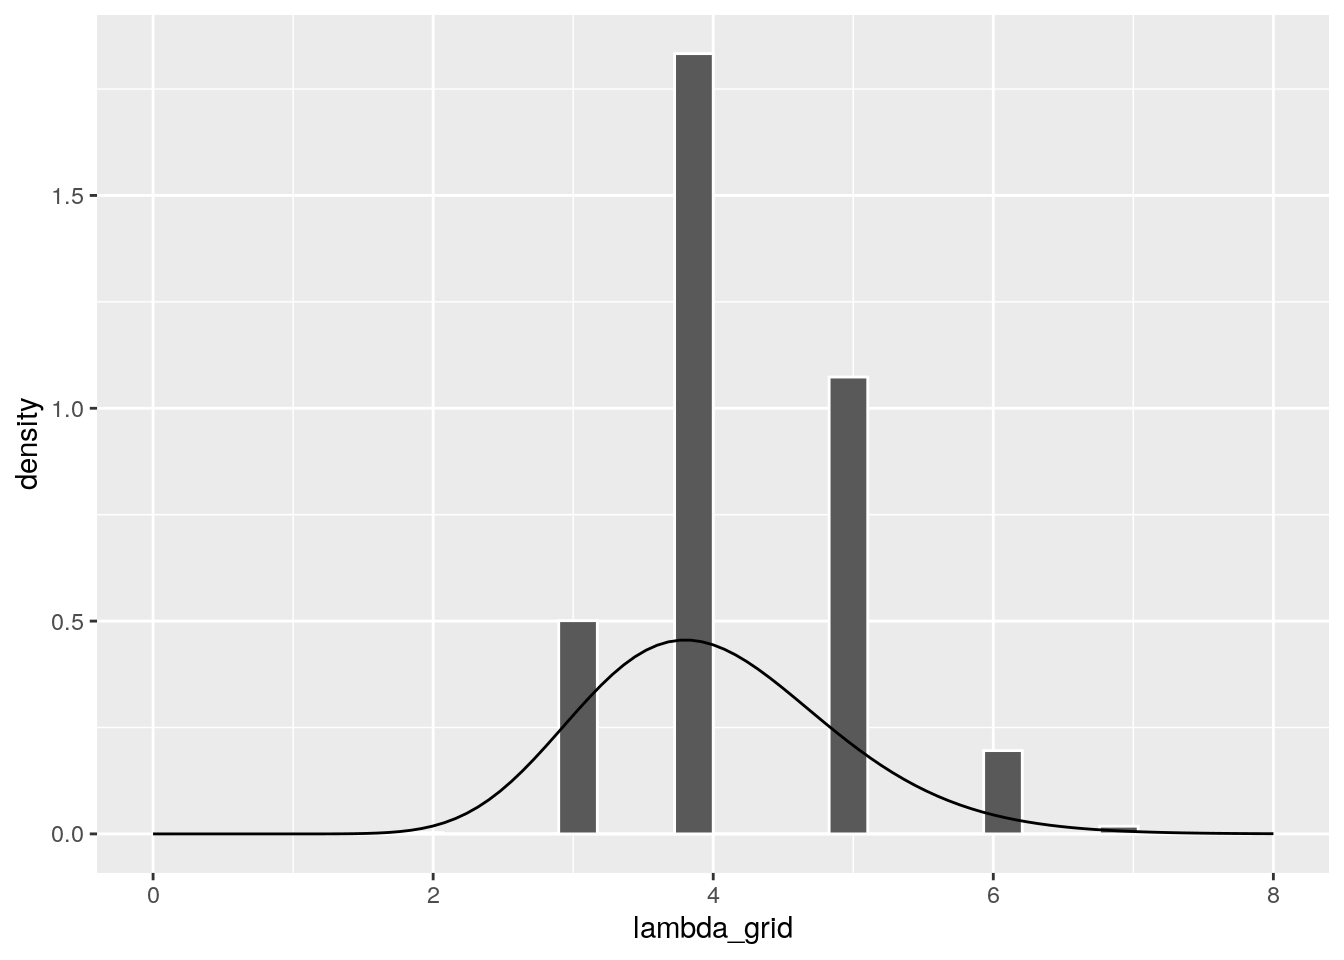
\includegraphics{ch9-10_files/figure-latex/unnamed-chunk-3-1.pdf}

\begin{Shaded}
\begin{Highlighting}[]
\CommentTok{\# Density plots of parallel chains}
\FunctionTok{mcmc\_dens\_overlay}\NormalTok{(model)}
\end{Highlighting}
\end{Shaded}

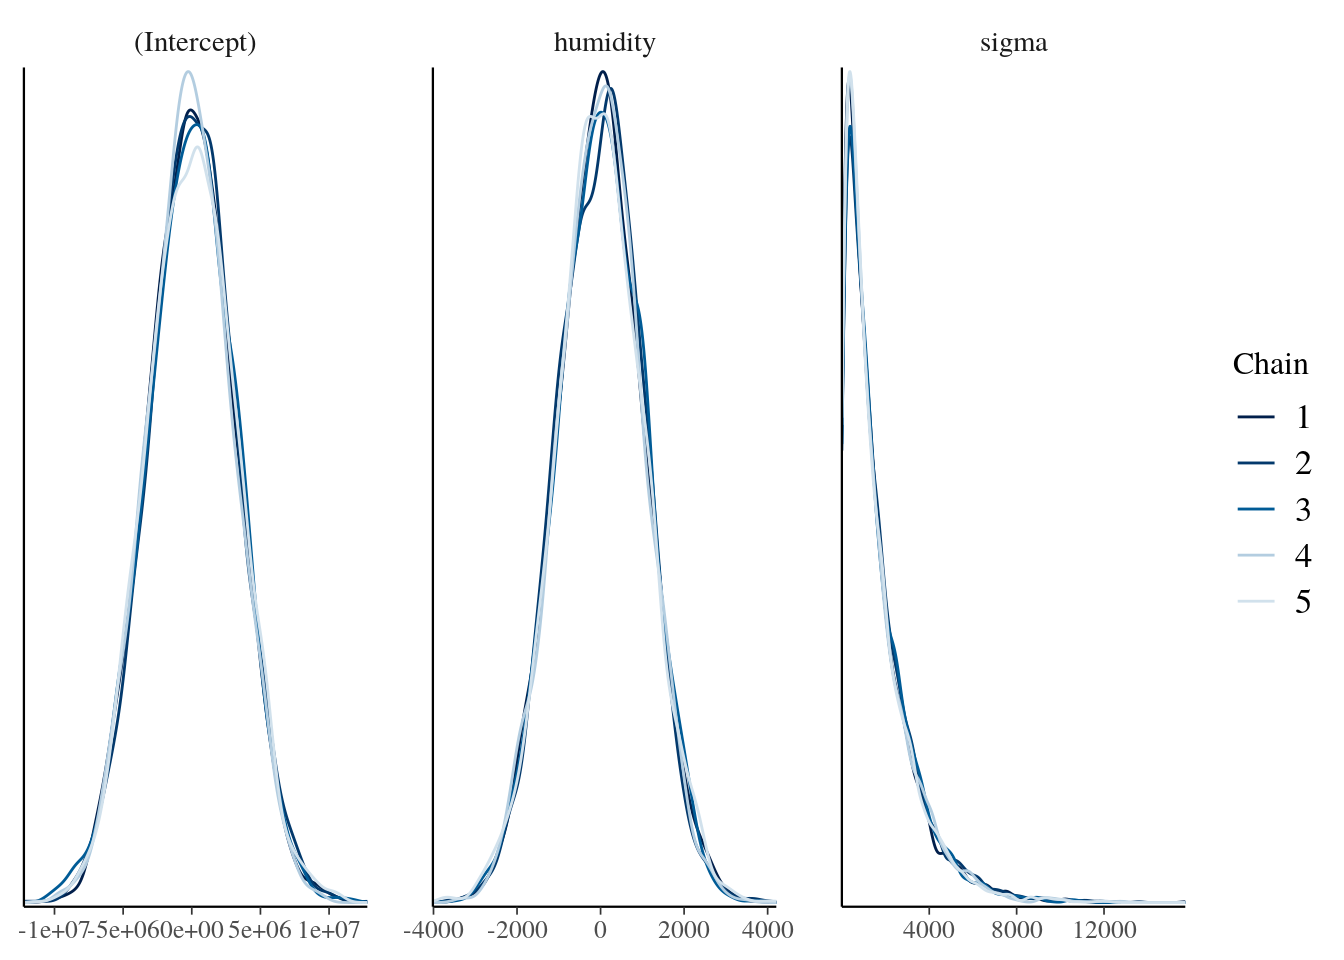
\includegraphics{ch9-10_files/figure-latex/unnamed-chunk-3-2.pdf}

\begin{enumerate}
\def\labelenumi{\alph{enumi}.}
\setcounter{enumi}{3}
\tightlist
\item
\end{enumerate}

Ridership decreases as humidity increases. There is much variability
with the ridership per day, so that impacts the strength of the
relationship.

\hypertarget{section-1}{%
\subsection{9.10}\label{section-1}}

\begin{enumerate}
\def\labelenumi{\alph{enumi}.}
\tightlist
\item
\end{enumerate}

\begin{Shaded}
\begin{Highlighting}[]
\CommentTok{\# Load and plot data}
\FunctionTok{data}\NormalTok{(bikes)}
\FunctionTok{ggplot}\NormalTok{(bikes, }\FunctionTok{aes}\NormalTok{(}\AttributeTok{x =}\NormalTok{ humidity, }\AttributeTok{y =}\NormalTok{ rides)) }\SpecialCharTok{+} 
  \FunctionTok{geom\_point}\NormalTok{(}\AttributeTok{size =} \FloatTok{0.5}\NormalTok{) }\SpecialCharTok{+} 
  \FunctionTok{geom\_smooth}\NormalTok{(}\AttributeTok{method =} \StringTok{"lm"}\NormalTok{, }\AttributeTok{se =} \ConstantTok{FALSE}\NormalTok{)}
\end{Highlighting}
\end{Shaded}

\begin{verbatim}
## `geom_smooth()` using formula 'y ~ x'
\end{verbatim}

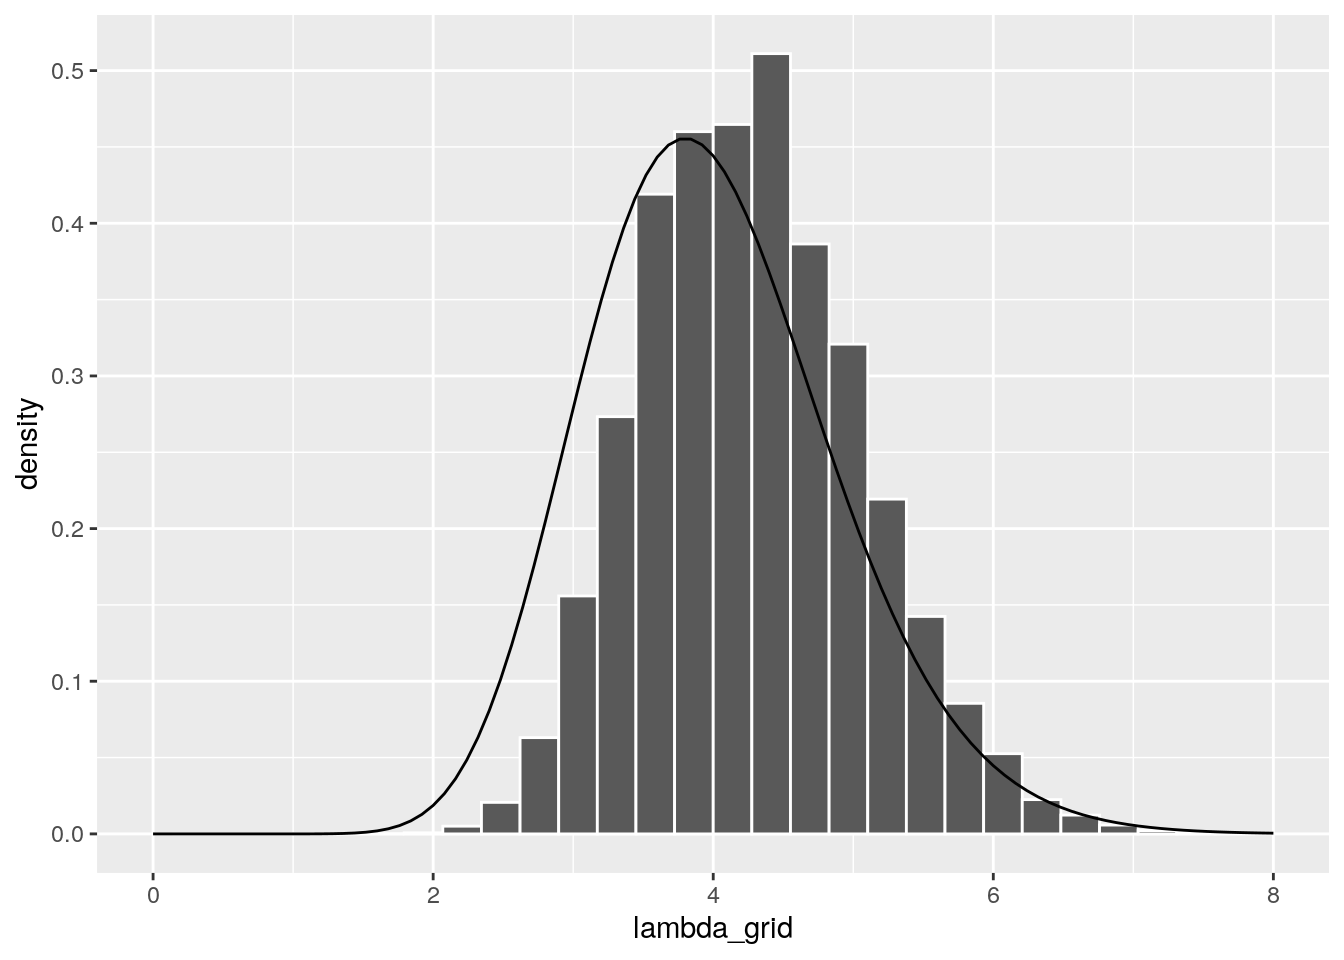
\includegraphics{ch9-10_files/figure-latex/unnamed-chunk-4-1.pdf}

\begin{enumerate}
\def\labelenumi{\alph{enumi}.}
\setcounter{enumi}{1}
\tightlist
\item
\end{enumerate}

The data is normally distributed enough; the points are fairly evenly
distributed across the y-axis. Since it doesn't form a trumpet-like
shape, it could be fine for Normal regression.

\hypertarget{section-2}{%
\subsection{9.11}\label{section-2}}

\begin{enumerate}
\def\labelenumi{\alph{enumi}.}
\tightlist
\item
\end{enumerate}

\begin{Shaded}
\begin{Highlighting}[]
\NormalTok{bike\_model }\OtherTok{\textless{}{-}} \FunctionTok{stan\_glm}\NormalTok{(rides }\SpecialCharTok{\textasciitilde{}}\NormalTok{ humidity, }\AttributeTok{data =}\NormalTok{ bikes, }
  \AttributeTok{family =}\NormalTok{ gaussian,}
  \AttributeTok{prior\_PD =} \ConstantTok{FALSE}\NormalTok{,}
  \AttributeTok{prior\_intercept =} \FunctionTok{normal}\NormalTok{(}\DecValTok{1000}\NormalTok{, }\DecValTok{2000}\NormalTok{, }\AttributeTok{autoscale =} \ConstantTok{TRUE}\NormalTok{),}
  \AttributeTok{prior =} \FunctionTok{normal}\NormalTok{(}\DecValTok{0}\NormalTok{, }\DecValTok{10}\NormalTok{, }\AttributeTok{autoscale =} \ConstantTok{TRUE}\NormalTok{), }
  \AttributeTok{prior\_aux =} \FunctionTok{exponential}\NormalTok{(}\DecValTok{1}\NormalTok{, }\AttributeTok{autoscale =} \ConstantTok{TRUE}\NormalTok{),}
  \AttributeTok{chains =} \DecValTok{5}\NormalTok{, }\AttributeTok{iter =} \DecValTok{4000}\SpecialCharTok{*}\DecValTok{2}\NormalTok{, }\AttributeTok{seed =} \DecValTok{84735}\NormalTok{)}
\end{Highlighting}
\end{Shaded}

\begin{verbatim}
## 
## SAMPLING FOR MODEL 'continuous' NOW (CHAIN 1).
## Chain 1: 
## Chain 1: Gradient evaluation took 2.7e-05 seconds
## Chain 1: 1000 transitions using 10 leapfrog steps per transition would take 0.27 seconds.
## Chain 1: Adjust your expectations accordingly!
## Chain 1: 
## Chain 1: 
## Chain 1: Iteration:    1 / 8000 [  0%]  (Warmup)
## Chain 1: Iteration:  800 / 8000 [ 10%]  (Warmup)
## Chain 1: Iteration: 1600 / 8000 [ 20%]  (Warmup)
## Chain 1: Iteration: 2400 / 8000 [ 30%]  (Warmup)
## Chain 1: Iteration: 3200 / 8000 [ 40%]  (Warmup)
## Chain 1: Iteration: 4000 / 8000 [ 50%]  (Warmup)
## Chain 1: Iteration: 4001 / 8000 [ 50%]  (Sampling)
## Chain 1: Iteration: 4800 / 8000 [ 60%]  (Sampling)
## Chain 1: Iteration: 5600 / 8000 [ 70%]  (Sampling)
## Chain 1: Iteration: 6400 / 8000 [ 80%]  (Sampling)
## Chain 1: Iteration: 7200 / 8000 [ 90%]  (Sampling)
## Chain 1: Iteration: 8000 / 8000 [100%]  (Sampling)
## Chain 1: 
## Chain 1:  Elapsed Time: 0.307736 seconds (Warm-up)
## Chain 1:                0.260575 seconds (Sampling)
## Chain 1:                0.568311 seconds (Total)
## Chain 1: 
## 
## SAMPLING FOR MODEL 'continuous' NOW (CHAIN 2).
## Chain 2: 
## Chain 2: Gradient evaluation took 8e-06 seconds
## Chain 2: 1000 transitions using 10 leapfrog steps per transition would take 0.08 seconds.
## Chain 2: Adjust your expectations accordingly!
## Chain 2: 
## Chain 2: 
## Chain 2: Iteration:    1 / 8000 [  0%]  (Warmup)
## Chain 2: Iteration:  800 / 8000 [ 10%]  (Warmup)
## Chain 2: Iteration: 1600 / 8000 [ 20%]  (Warmup)
## Chain 2: Iteration: 2400 / 8000 [ 30%]  (Warmup)
## Chain 2: Iteration: 3200 / 8000 [ 40%]  (Warmup)
## Chain 2: Iteration: 4000 / 8000 [ 50%]  (Warmup)
## Chain 2: Iteration: 4001 / 8000 [ 50%]  (Sampling)
## Chain 2: Iteration: 4800 / 8000 [ 60%]  (Sampling)
## Chain 2: Iteration: 5600 / 8000 [ 70%]  (Sampling)
## Chain 2: Iteration: 6400 / 8000 [ 80%]  (Sampling)
## Chain 2: Iteration: 7200 / 8000 [ 90%]  (Sampling)
## Chain 2: Iteration: 8000 / 8000 [100%]  (Sampling)
## Chain 2: 
## Chain 2:  Elapsed Time: 0.341191 seconds (Warm-up)
## Chain 2:                0.261191 seconds (Sampling)
## Chain 2:                0.602382 seconds (Total)
## Chain 2: 
## 
## SAMPLING FOR MODEL 'continuous' NOW (CHAIN 3).
## Chain 3: 
## Chain 3: Gradient evaluation took 9e-06 seconds
## Chain 3: 1000 transitions using 10 leapfrog steps per transition would take 0.09 seconds.
## Chain 3: Adjust your expectations accordingly!
## Chain 3: 
## Chain 3: 
## Chain 3: Iteration:    1 / 8000 [  0%]  (Warmup)
## Chain 3: Iteration:  800 / 8000 [ 10%]  (Warmup)
## Chain 3: Iteration: 1600 / 8000 [ 20%]  (Warmup)
## Chain 3: Iteration: 2400 / 8000 [ 30%]  (Warmup)
## Chain 3: Iteration: 3200 / 8000 [ 40%]  (Warmup)
## Chain 3: Iteration: 4000 / 8000 [ 50%]  (Warmup)
## Chain 3: Iteration: 4001 / 8000 [ 50%]  (Sampling)
## Chain 3: Iteration: 4800 / 8000 [ 60%]  (Sampling)
## Chain 3: Iteration: 5600 / 8000 [ 70%]  (Sampling)
## Chain 3: Iteration: 6400 / 8000 [ 80%]  (Sampling)
## Chain 3: Iteration: 7200 / 8000 [ 90%]  (Sampling)
## Chain 3: Iteration: 8000 / 8000 [100%]  (Sampling)
## Chain 3: 
## Chain 3:  Elapsed Time: 0.222038 seconds (Warm-up)
## Chain 3:                0.262781 seconds (Sampling)
## Chain 3:                0.484819 seconds (Total)
## Chain 3: 
## 
## SAMPLING FOR MODEL 'continuous' NOW (CHAIN 4).
## Chain 4: 
## Chain 4: Gradient evaluation took 8e-06 seconds
## Chain 4: 1000 transitions using 10 leapfrog steps per transition would take 0.08 seconds.
## Chain 4: Adjust your expectations accordingly!
## Chain 4: 
## Chain 4: 
## Chain 4: Iteration:    1 / 8000 [  0%]  (Warmup)
## Chain 4: Iteration:  800 / 8000 [ 10%]  (Warmup)
## Chain 4: Iteration: 1600 / 8000 [ 20%]  (Warmup)
## Chain 4: Iteration: 2400 / 8000 [ 30%]  (Warmup)
## Chain 4: Iteration: 3200 / 8000 [ 40%]  (Warmup)
## Chain 4: Iteration: 4000 / 8000 [ 50%]  (Warmup)
## Chain 4: Iteration: 4001 / 8000 [ 50%]  (Sampling)
## Chain 4: Iteration: 4800 / 8000 [ 60%]  (Sampling)
## Chain 4: Iteration: 5600 / 8000 [ 70%]  (Sampling)
## Chain 4: Iteration: 6400 / 8000 [ 80%]  (Sampling)
## Chain 4: Iteration: 7200 / 8000 [ 90%]  (Sampling)
## Chain 4: Iteration: 8000 / 8000 [100%]  (Sampling)
## Chain 4: 
## Chain 4:  Elapsed Time: 1.65368 seconds (Warm-up)
## Chain 4:                0.263492 seconds (Sampling)
## Chain 4:                1.91717 seconds (Total)
## Chain 4: 
## 
## SAMPLING FOR MODEL 'continuous' NOW (CHAIN 5).
## Chain 5: 
## Chain 5: Gradient evaluation took 9e-06 seconds
## Chain 5: 1000 transitions using 10 leapfrog steps per transition would take 0.09 seconds.
## Chain 5: Adjust your expectations accordingly!
## Chain 5: 
## Chain 5: 
## Chain 5: Iteration:    1 / 8000 [  0%]  (Warmup)
## Chain 5: Iteration:  800 / 8000 [ 10%]  (Warmup)
## Chain 5: Iteration: 1600 / 8000 [ 20%]  (Warmup)
## Chain 5: Iteration: 2400 / 8000 [ 30%]  (Warmup)
## Chain 5: Iteration: 3200 / 8000 [ 40%]  (Warmup)
## Chain 5: Iteration: 4000 / 8000 [ 50%]  (Warmup)
## Chain 5: Iteration: 4001 / 8000 [ 50%]  (Sampling)
## Chain 5: Iteration: 4800 / 8000 [ 60%]  (Sampling)
## Chain 5: Iteration: 5600 / 8000 [ 70%]  (Sampling)
## Chain 5: Iteration: 6400 / 8000 [ 80%]  (Sampling)
## Chain 5: Iteration: 7200 / 8000 [ 90%]  (Sampling)
## Chain 5: Iteration: 8000 / 8000 [100%]  (Sampling)
## Chain 5: 
## Chain 5:  Elapsed Time: 0.164299 seconds (Warm-up)
## Chain 5:                0.276779 seconds (Sampling)
## Chain 5:                0.441078 seconds (Total)
## Chain 5:
\end{verbatim}

\begin{enumerate}
\def\labelenumi{\alph{enumi}.}
\setcounter{enumi}{1}
\tightlist
\item
\end{enumerate}

\begin{Shaded}
\begin{Highlighting}[]
\CommentTok{\# Effective sample size ratio }
\FunctionTok{neff\_ratio}\NormalTok{(bike\_model)}
\end{Highlighting}
\end{Shaded}

\begin{verbatim}
## (Intercept)    humidity       sigma 
##     0.99525     0.99270     0.96705
\end{verbatim}

\begin{Shaded}
\begin{Highlighting}[]
\CommentTok{\# Density plots of parallel chains}
\FunctionTok{mcmc\_dens\_overlay}\NormalTok{(bike\_model)}
\end{Highlighting}
\end{Shaded}

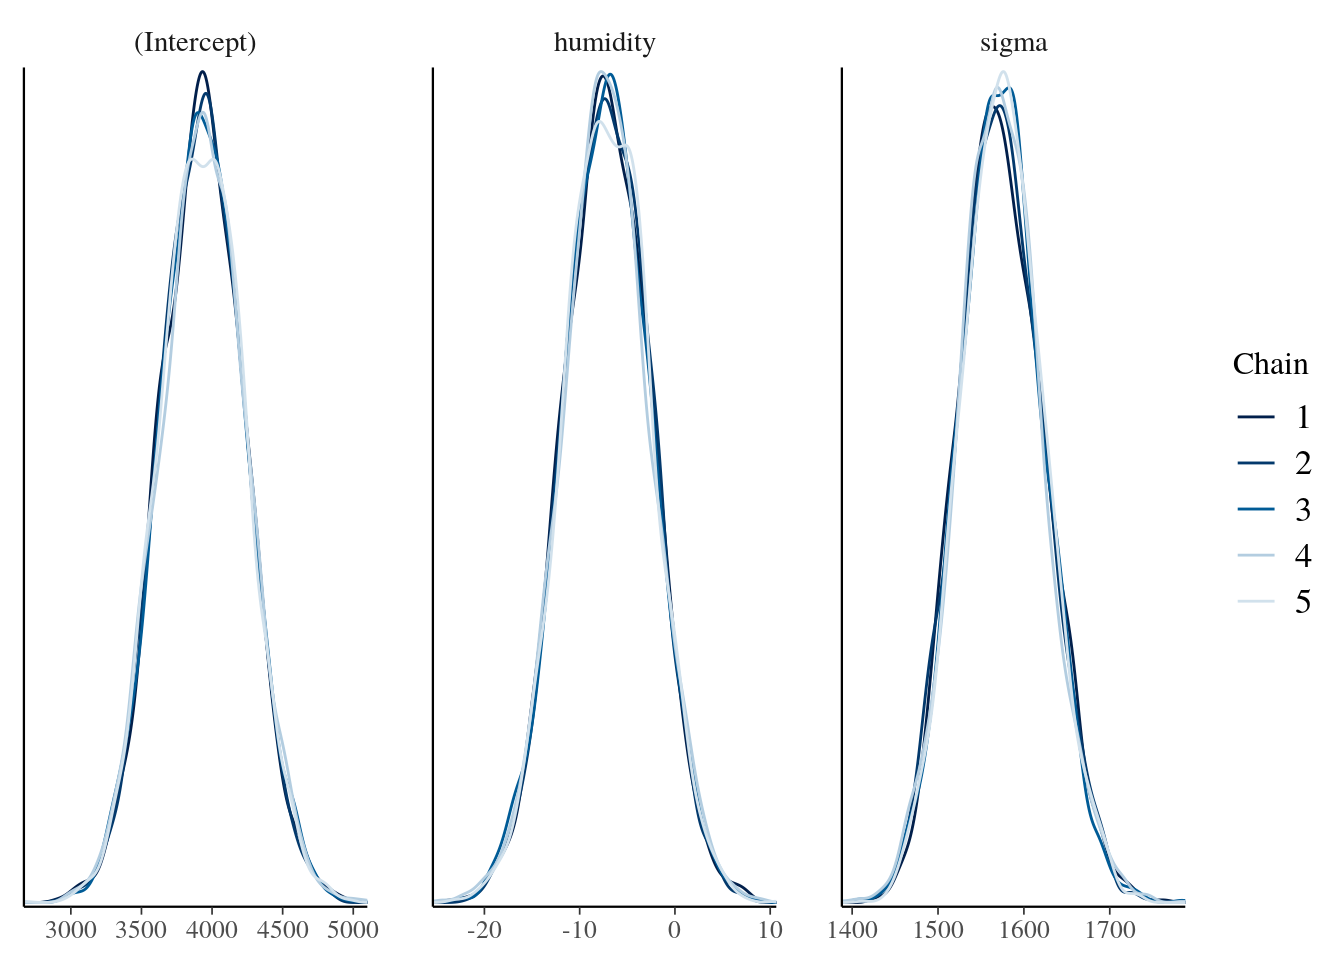
\includegraphics{ch9-10_files/figure-latex/unnamed-chunk-7-1.pdf}

Given the results above, we can trust these simulation results.

\begin{enumerate}
\def\labelenumi{\alph{enumi}.}
\setcounter{enumi}{2}
\tightlist
\item
\end{enumerate}

\begin{Shaded}
\begin{Highlighting}[]
\CommentTok{\# Trace plots of parallel chains}
\FunctionTok{mcmc\_trace}\NormalTok{(bike\_model, }\AttributeTok{size =}\NormalTok{ .}\DecValTok{1}\NormalTok{)}
\end{Highlighting}
\end{Shaded}

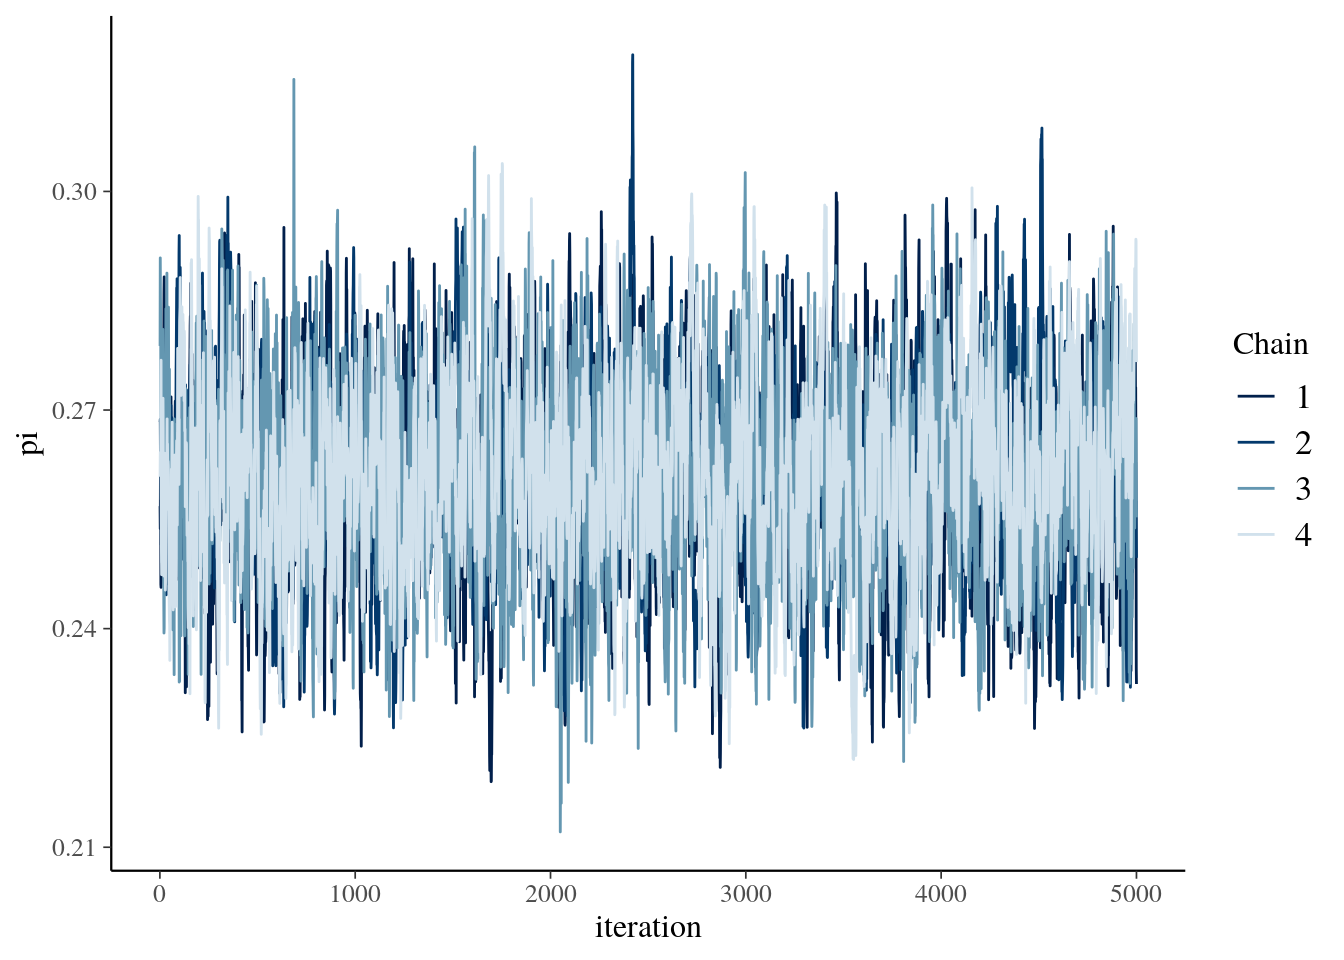
\includegraphics{ch9-10_files/figure-latex/unnamed-chunk-8-1.pdf}

The sigma is more centered than 9.9's and the scales are much different.

\hypertarget{section-3}{%
\subsection{9.12}\label{section-3}}

\begin{enumerate}
\def\labelenumi{\alph{enumi}.}
\tightlist
\item
\end{enumerate}

\begin{Shaded}
\begin{Highlighting}[]
\FunctionTok{tidy}\NormalTok{(bike\_model, }\AttributeTok{effects =} \FunctionTok{c}\NormalTok{(}\StringTok{"fixed"}\NormalTok{, }\StringTok{"aux"}\NormalTok{),}
     \AttributeTok{conf.int =} \ConstantTok{TRUE}\NormalTok{, }\AttributeTok{conf.level =} \FloatTok{0.95}\NormalTok{)}
\end{Highlighting}
\end{Shaded}

\begin{verbatim}
## # A tibble: 4 x 5
##   term        estimate std.error conf.low conf.high
##   <chr>          <dbl>     <dbl>    <dbl>     <dbl>
## 1 (Intercept)  3935.      303.     3342.    4534.  
## 2 humidity       -7.13      4.64    -16.2      1.90
## 3 sigma        1573.       49.7    1480.    1676.  
## 4 mean_PPD     3483.      100.     3284.    3678.
\end{verbatim}

\begin{enumerate}
\def\labelenumi{\alph{enumi}.}
\setcounter{enumi}{1}
\tightlist
\item
\end{enumerate}

The posterior median relationship is 3935.315 - 8.128. That means for
every one degree increase in humidity, we expect ridership to decrease
by about 8 rides.

\begin{enumerate}
\def\labelenumi{\alph{enumi}.}
\setcounter{enumi}{2}
\tightlist
\item
\end{enumerate}

The CI represents the uncertainty in the relationship. \[\beta_1\]
(-16.16035,1.899641) indicates that this slope could range anywhere
between about -16 and 2.

\begin{enumerate}
\def\labelenumi{\alph{enumi}.}
\setcounter{enumi}{3}
\tightlist
\item
\end{enumerate}

I would say that we have alright posterior evidence that there's a
negative association between ridership and humidity. The standard error
is low enough for it to carry some weight, but not low enough for there
to be very certain evidence to their relationship. However, the CI is a
small range, so that does help the credibility of the evidence of their
relationship.

\hypertarget{section-4}{%
\subsection{9.16}\label{section-4}}

\begin{enumerate}
\def\labelenumi{\alph{enumi}.}
\tightlist
\item
\end{enumerate}

\begin{Shaded}
\begin{Highlighting}[]
\FunctionTok{summary}\NormalTok{(penguins\_bayes)}
\end{Highlighting}
\end{Shaded}

\begin{verbatim}
##       species          island         year      bill_length_mm  bill_depth_mm  
##  Adelie   :152   Biscoe   :168   Min.   :2007   Min.   :32.10   Min.   :13.10  
##  Chinstrap: 68   Dream    :124   1st Qu.:2007   1st Qu.:39.23   1st Qu.:15.60  
##  Gentoo   :124   Torgersen: 52   Median :2008   Median :44.45   Median :17.30  
##                                  Mean   :2008   Mean   :43.92   Mean   :17.15  
##                                  3rd Qu.:2009   3rd Qu.:48.50   3rd Qu.:18.70  
##                                  Max.   :2009   Max.   :59.60   Max.   :21.50  
##                                                 NA's   :2       NA's   :2      
##  flipper_length_mm  body_mass_g   above_average_weight     sex     
##  Min.   :172.0     Min.   :2700   0   :193             female:165  
##  1st Qu.:190.0     1st Qu.:3550   1   :149             male  :168  
##  Median :197.0     Median :4050   NA's:  2             NA's  : 11  
##  Mean   :200.9     Mean   :4202                                    
##  3rd Qu.:213.0     3rd Qu.:4750                                    
##  Max.   :231.0     Max.   :6300                                    
##  NA's   :2         NA's   :2
\end{verbatim}

\begin{Shaded}
\begin{Highlighting}[]
\NormalTok{penguins\_model }\OtherTok{\textless{}{-}} \FunctionTok{stan\_glm}\NormalTok{(flipper\_length\_mm }\SpecialCharTok{\textasciitilde{}}\NormalTok{ bill\_length\_mm, }\AttributeTok{data =}\NormalTok{ penguins\_bayes,}
                       \AttributeTok{family =}\NormalTok{ gaussian,}
                       \AttributeTok{prior\_PD =} \ConstantTok{TRUE}\NormalTok{, }
                       \AttributeTok{prior\_intercept =} \FunctionTok{normal}\NormalTok{(}\FloatTok{43.92}\NormalTok{, }\FloatTok{11.82}\NormalTok{),}
                       \AttributeTok{prior =} \FunctionTok{normal}\NormalTok{(}\FloatTok{200.9}\NormalTok{, }\FloatTok{28.9}\NormalTok{), }
                       \AttributeTok{prior\_aux =} \FunctionTok{exponential}\NormalTok{(}\FloatTok{0.0008}\NormalTok{),}
                       \AttributeTok{chains =} \DecValTok{4}\NormalTok{, }\AttributeTok{iter =} \DecValTok{10000}\SpecialCharTok{*}\DecValTok{2}\NormalTok{, }\AttributeTok{seed =} \DecValTok{84735}\NormalTok{)}
\end{Highlighting}
\end{Shaded}

\begin{verbatim}
## 
## SAMPLING FOR MODEL 'continuous' NOW (CHAIN 1).
## Chain 1: 
## Chain 1: Gradient evaluation took 1.6e-05 seconds
## Chain 1: 1000 transitions using 10 leapfrog steps per transition would take 0.16 seconds.
## Chain 1: Adjust your expectations accordingly!
## Chain 1: 
## Chain 1: 
## Chain 1: Iteration:     1 / 20000 [  0%]  (Warmup)
## Chain 1: Iteration:  2000 / 20000 [ 10%]  (Warmup)
## Chain 1: Iteration:  4000 / 20000 [ 20%]  (Warmup)
## Chain 1: Iteration:  6000 / 20000 [ 30%]  (Warmup)
## Chain 1: Iteration:  8000 / 20000 [ 40%]  (Warmup)
## Chain 1: Iteration: 10000 / 20000 [ 50%]  (Warmup)
## Chain 1: Iteration: 10001 / 20000 [ 50%]  (Sampling)
## Chain 1: Iteration: 12000 / 20000 [ 60%]  (Sampling)
## Chain 1: Iteration: 14000 / 20000 [ 70%]  (Sampling)
## Chain 1: Iteration: 16000 / 20000 [ 80%]  (Sampling)
## Chain 1: Iteration: 18000 / 20000 [ 90%]  (Sampling)
## Chain 1: Iteration: 20000 / 20000 [100%]  (Sampling)
## Chain 1: 
## Chain 1:  Elapsed Time: 0.174128 seconds (Warm-up)
## Chain 1:                0.248485 seconds (Sampling)
## Chain 1:                0.422613 seconds (Total)
## Chain 1: 
## 
## SAMPLING FOR MODEL 'continuous' NOW (CHAIN 2).
## Chain 2: 
## Chain 2: Gradient evaluation took 9e-06 seconds
## Chain 2: 1000 transitions using 10 leapfrog steps per transition would take 0.09 seconds.
## Chain 2: Adjust your expectations accordingly!
## Chain 2: 
## Chain 2: 
## Chain 2: Iteration:     1 / 20000 [  0%]  (Warmup)
## Chain 2: Iteration:  2000 / 20000 [ 10%]  (Warmup)
## Chain 2: Iteration:  4000 / 20000 [ 20%]  (Warmup)
## Chain 2: Iteration:  6000 / 20000 [ 30%]  (Warmup)
## Chain 2: Iteration:  8000 / 20000 [ 40%]  (Warmup)
## Chain 2: Iteration: 10000 / 20000 [ 50%]  (Warmup)
## Chain 2: Iteration: 10001 / 20000 [ 50%]  (Sampling)
## Chain 2: Iteration: 12000 / 20000 [ 60%]  (Sampling)
## Chain 2: Iteration: 14000 / 20000 [ 70%]  (Sampling)
## Chain 2: Iteration: 16000 / 20000 [ 80%]  (Sampling)
## Chain 2: Iteration: 18000 / 20000 [ 90%]  (Sampling)
## Chain 2: Iteration: 20000 / 20000 [100%]  (Sampling)
## Chain 2: 
## Chain 2:  Elapsed Time: 0.175503 seconds (Warm-up)
## Chain 2:                0.181991 seconds (Sampling)
## Chain 2:                0.357494 seconds (Total)
## Chain 2: 
## 
## SAMPLING FOR MODEL 'continuous' NOW (CHAIN 3).
## Chain 3: 
## Chain 3: Gradient evaluation took 7e-06 seconds
## Chain 3: 1000 transitions using 10 leapfrog steps per transition would take 0.07 seconds.
## Chain 3: Adjust your expectations accordingly!
## Chain 3: 
## Chain 3: 
## Chain 3: Iteration:     1 / 20000 [  0%]  (Warmup)
## Chain 3: Iteration:  2000 / 20000 [ 10%]  (Warmup)
## Chain 3: Iteration:  4000 / 20000 [ 20%]  (Warmup)
## Chain 3: Iteration:  6000 / 20000 [ 30%]  (Warmup)
## Chain 3: Iteration:  8000 / 20000 [ 40%]  (Warmup)
## Chain 3: Iteration: 10000 / 20000 [ 50%]  (Warmup)
## Chain 3: Iteration: 10001 / 20000 [ 50%]  (Sampling)
## Chain 3: Iteration: 12000 / 20000 [ 60%]  (Sampling)
## Chain 3: Iteration: 14000 / 20000 [ 70%]  (Sampling)
## Chain 3: Iteration: 16000 / 20000 [ 80%]  (Sampling)
## Chain 3: Iteration: 18000 / 20000 [ 90%]  (Sampling)
## Chain 3: Iteration: 20000 / 20000 [100%]  (Sampling)
## Chain 3: 
## Chain 3:  Elapsed Time: 0.178473 seconds (Warm-up)
## Chain 3:                0.239264 seconds (Sampling)
## Chain 3:                0.417737 seconds (Total)
## Chain 3: 
## 
## SAMPLING FOR MODEL 'continuous' NOW (CHAIN 4).
## Chain 4: 
## Chain 4: Gradient evaluation took 5e-06 seconds
## Chain 4: 1000 transitions using 10 leapfrog steps per transition would take 0.05 seconds.
## Chain 4: Adjust your expectations accordingly!
## Chain 4: 
## Chain 4: 
## Chain 4: Iteration:     1 / 20000 [  0%]  (Warmup)
## Chain 4: Iteration:  2000 / 20000 [ 10%]  (Warmup)
## Chain 4: Iteration:  4000 / 20000 [ 20%]  (Warmup)
## Chain 4: Iteration:  6000 / 20000 [ 30%]  (Warmup)
## Chain 4: Iteration:  8000 / 20000 [ 40%]  (Warmup)
## Chain 4: Iteration: 10000 / 20000 [ 50%]  (Warmup)
## Chain 4: Iteration: 10001 / 20000 [ 50%]  (Sampling)
## Chain 4: Iteration: 12000 / 20000 [ 60%]  (Sampling)
## Chain 4: Iteration: 14000 / 20000 [ 70%]  (Sampling)
## Chain 4: Iteration: 16000 / 20000 [ 80%]  (Sampling)
## Chain 4: Iteration: 18000 / 20000 [ 90%]  (Sampling)
## Chain 4: Iteration: 20000 / 20000 [100%]  (Sampling)
## Chain 4: 
## Chain 4:  Elapsed Time: 0.177074 seconds (Warm-up)
## Chain 4:                0.238337 seconds (Sampling)
## Chain 4:                0.415411 seconds (Total)
## Chain 4:
\end{verbatim}

\begin{enumerate}
\def\labelenumi{\alph{enumi}.}
\setcounter{enumi}{1}
\tightlist
\item
\end{enumerate}

\begin{Shaded}
\begin{Highlighting}[]
\FunctionTok{prior\_summary}\NormalTok{(penguins\_model)}
\end{Highlighting}
\end{Shaded}

\begin{verbatim}
## Priors for model 'penguins_model' 
## ------
## Intercept (after predictors centered)
##  ~ normal(location = 44, scale = 12)
## 
## Coefficients
##  ~ normal(location = 201, scale = 29)
## 
## Auxiliary (sigma)
##  ~ exponential(rate = 8e-04)
## ------
## See help('prior_summary.stanreg') for more details
\end{verbatim}

\begin{enumerate}
\def\labelenumi{\alph{enumi}.}
\setcounter{enumi}{2}
\tightlist
\item
\end{enumerate}

\begin{Shaded}
\begin{Highlighting}[]
\CommentTok{\# Trace plots of parallel chains}
\FunctionTok{mcmc\_trace}\NormalTok{(penguins\_model, }\AttributeTok{size =} \FloatTok{0.1}\NormalTok{)}
\end{Highlighting}
\end{Shaded}

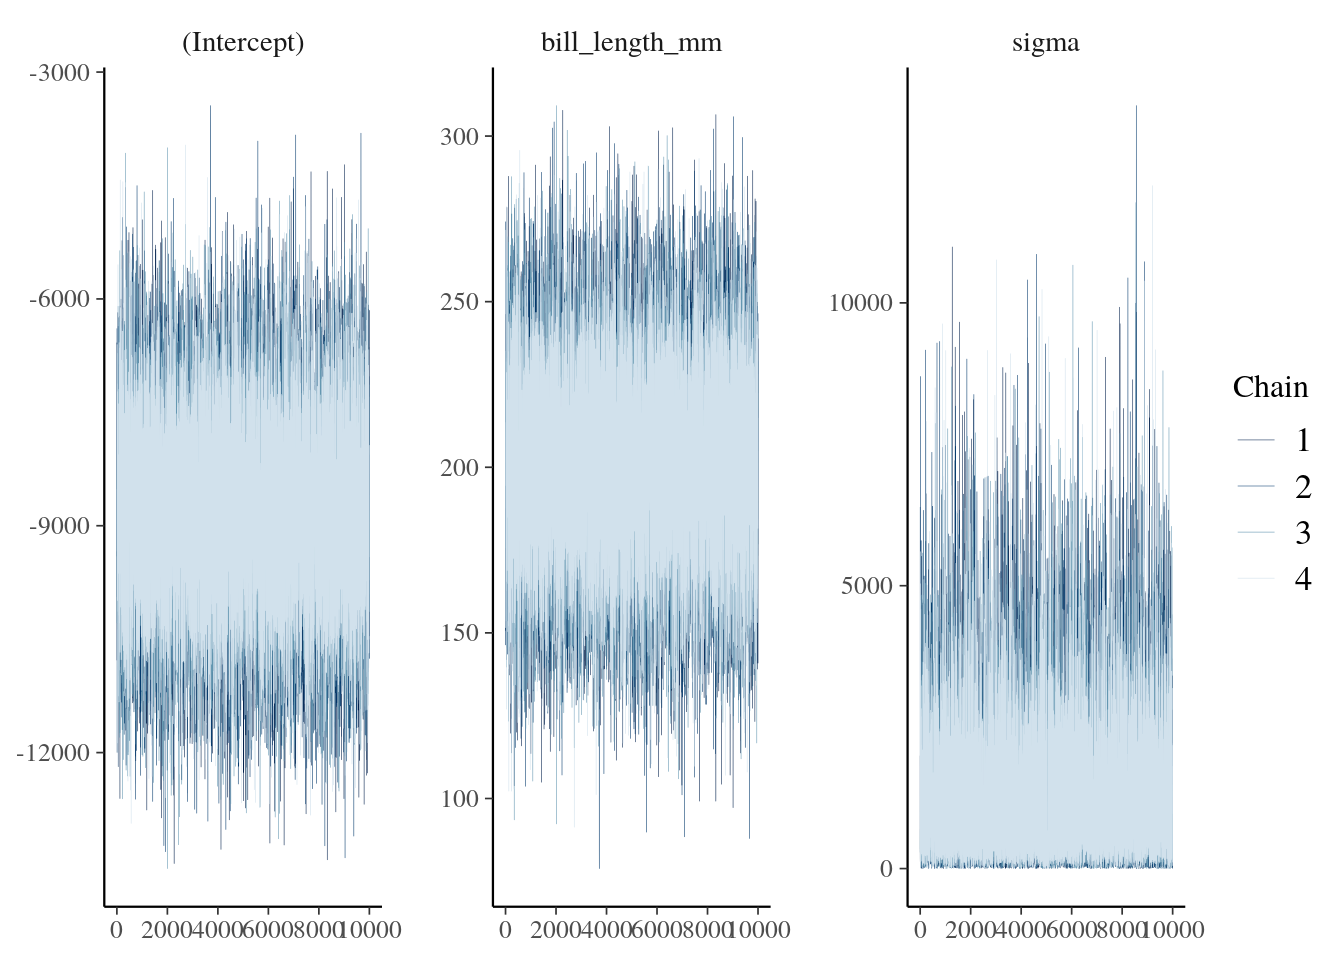
\includegraphics{ch9-10_files/figure-latex/unnamed-chunk-13-1.pdf}

\begin{enumerate}
\def\labelenumi{\alph{enumi}.}
\setcounter{enumi}{3}
\tightlist
\item
\end{enumerate}

It looks like flipper and bill length may be negatively associated.

\hypertarget{section-5}{%
\subsection{9.17}\label{section-5}}

\begin{enumerate}
\def\labelenumi{\alph{enumi}.}
\tightlist
\item
\end{enumerate}

\begin{Shaded}
\begin{Highlighting}[]
\NormalTok{penguins\_bayes }\SpecialCharTok{|\textgreater{}}
  \FunctionTok{ggplot}\NormalTok{(}\FunctionTok{aes}\NormalTok{(}\AttributeTok{x =}\NormalTok{ flipper\_length\_mm, }\AttributeTok{y =}\NormalTok{ bill\_length\_mm)) }\SpecialCharTok{+}
  \FunctionTok{geom\_point}\NormalTok{()}
\end{Highlighting}
\end{Shaded}

\begin{verbatim}
## Warning: Removed 2 rows containing missing values (geom_point).
\end{verbatim}

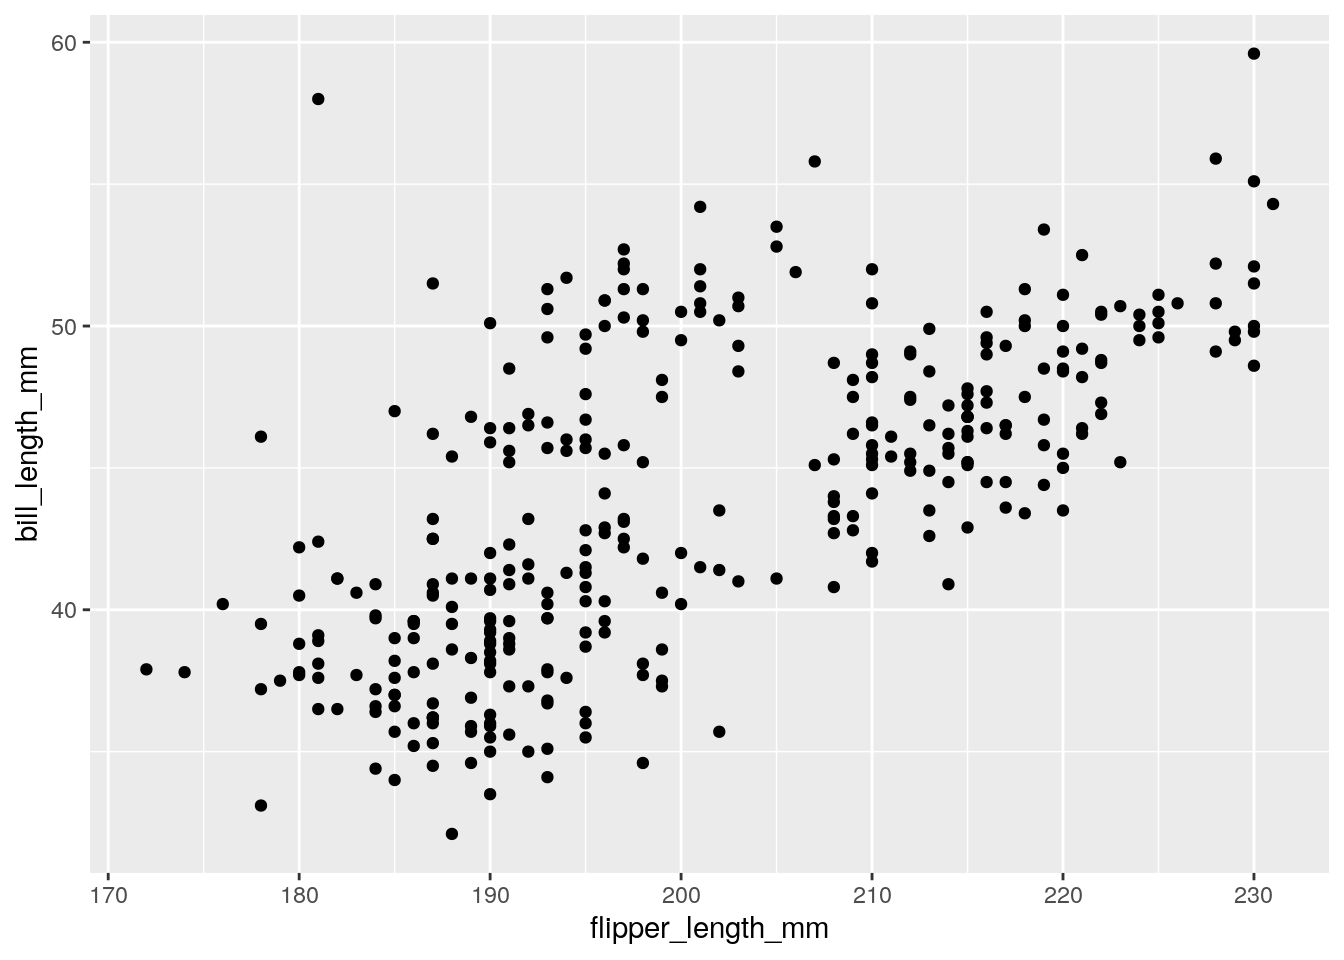
\includegraphics{ch9-10_files/figure-latex/unnamed-chunk-14-1.pdf}

There appears to be a positive linear relationship between flipper and
bill length.

\begin{enumerate}
\def\labelenumi{\alph{enumi}.}
\setcounter{enumi}{1}
\tightlist
\item
\end{enumerate}

It meets the conditions for a simple normal regression model. It has
linearity on the plot above. If it also has independent observations and
is normally distributed on a fitted vs resids plot, we can use a normal
model.

\hypertarget{section-6}{%
\subsection{9.18}\label{section-6}}

\begin{enumerate}
\def\labelenumi{\alph{enumi}.}
\tightlist
\item
\end{enumerate}

\begin{Shaded}
\begin{Highlighting}[]
\NormalTok{penguins\_post\_model }\OtherTok{\textless{}{-}} \FunctionTok{stan\_glm}\NormalTok{(flipper\_length\_mm }\SpecialCharTok{\textasciitilde{}}\NormalTok{ bill\_length\_mm, }\AttributeTok{data =}\NormalTok{ penguins\_bayes,}
                       \AttributeTok{family =}\NormalTok{ gaussian,}
                       \AttributeTok{prior\_intercept =} \FunctionTok{normal}\NormalTok{(}\FloatTok{43.92}\NormalTok{, }\FloatTok{11.82}\NormalTok{),}
                       \AttributeTok{prior =} \FunctionTok{normal}\NormalTok{(}\FloatTok{200.9}\NormalTok{, }\FloatTok{28.9}\NormalTok{), }
                       \AttributeTok{prior\_aux =} \FunctionTok{exponential}\NormalTok{(}\FloatTok{0.0008}\NormalTok{),}
                       \AttributeTok{chains =} \DecValTok{4}\NormalTok{, }\AttributeTok{iter =} \DecValTok{10000}\SpecialCharTok{*}\DecValTok{2}\NormalTok{, }\AttributeTok{seed =} \DecValTok{84735}\NormalTok{)}
\end{Highlighting}
\end{Shaded}

\begin{verbatim}
## 
## SAMPLING FOR MODEL 'continuous' NOW (CHAIN 1).
## Chain 1: 
## Chain 1: Gradient evaluation took 2.5e-05 seconds
## Chain 1: 1000 transitions using 10 leapfrog steps per transition would take 0.25 seconds.
## Chain 1: Adjust your expectations accordingly!
## Chain 1: 
## Chain 1: 
## Chain 1: Iteration:     1 / 20000 [  0%]  (Warmup)
## Chain 1: Iteration:  2000 / 20000 [ 10%]  (Warmup)
## Chain 1: Iteration:  4000 / 20000 [ 20%]  (Warmup)
## Chain 1: Iteration:  6000 / 20000 [ 30%]  (Warmup)
## Chain 1: Iteration:  8000 / 20000 [ 40%]  (Warmup)
## Chain 1: Iteration: 10000 / 20000 [ 50%]  (Warmup)
## Chain 1: Iteration: 10001 / 20000 [ 50%]  (Sampling)
## Chain 1: Iteration: 12000 / 20000 [ 60%]  (Sampling)
## Chain 1: Iteration: 14000 / 20000 [ 70%]  (Sampling)
## Chain 1: Iteration: 16000 / 20000 [ 80%]  (Sampling)
## Chain 1: Iteration: 18000 / 20000 [ 90%]  (Sampling)
## Chain 1: Iteration: 20000 / 20000 [100%]  (Sampling)
## Chain 1: 
## Chain 1:  Elapsed Time: 0.222189 seconds (Warm-up)
## Chain 1:                0.599516 seconds (Sampling)
## Chain 1:                0.821705 seconds (Total)
## Chain 1: 
## 
## SAMPLING FOR MODEL 'continuous' NOW (CHAIN 2).
## Chain 2: 
## Chain 2: Gradient evaluation took 9e-06 seconds
## Chain 2: 1000 transitions using 10 leapfrog steps per transition would take 0.09 seconds.
## Chain 2: Adjust your expectations accordingly!
## Chain 2: 
## Chain 2: 
## Chain 2: Iteration:     1 / 20000 [  0%]  (Warmup)
## Chain 2: Iteration:  2000 / 20000 [ 10%]  (Warmup)
## Chain 2: Iteration:  4000 / 20000 [ 20%]  (Warmup)
## Chain 2: Iteration:  6000 / 20000 [ 30%]  (Warmup)
## Chain 2: Iteration:  8000 / 20000 [ 40%]  (Warmup)
## Chain 2: Iteration: 10000 / 20000 [ 50%]  (Warmup)
## Chain 2: Iteration: 10001 / 20000 [ 50%]  (Sampling)
## Chain 2: Iteration: 12000 / 20000 [ 60%]  (Sampling)
## Chain 2: Iteration: 14000 / 20000 [ 70%]  (Sampling)
## Chain 2: Iteration: 16000 / 20000 [ 80%]  (Sampling)
## Chain 2: Iteration: 18000 / 20000 [ 90%]  (Sampling)
## Chain 2: Iteration: 20000 / 20000 [100%]  (Sampling)
## Chain 2: 
## Chain 2:  Elapsed Time: 0.22647 seconds (Warm-up)
## Chain 2:                0.580577 seconds (Sampling)
## Chain 2:                0.807047 seconds (Total)
## Chain 2: 
## 
## SAMPLING FOR MODEL 'continuous' NOW (CHAIN 3).
## Chain 3: 
## Chain 3: Gradient evaluation took 9e-06 seconds
## Chain 3: 1000 transitions using 10 leapfrog steps per transition would take 0.09 seconds.
## Chain 3: Adjust your expectations accordingly!
## Chain 3: 
## Chain 3: 
## Chain 3: Iteration:     1 / 20000 [  0%]  (Warmup)
## Chain 3: Iteration:  2000 / 20000 [ 10%]  (Warmup)
## Chain 3: Iteration:  4000 / 20000 [ 20%]  (Warmup)
## Chain 3: Iteration:  6000 / 20000 [ 30%]  (Warmup)
## Chain 3: Iteration:  8000 / 20000 [ 40%]  (Warmup)
## Chain 3: Iteration: 10000 / 20000 [ 50%]  (Warmup)
## Chain 3: Iteration: 10001 / 20000 [ 50%]  (Sampling)
## Chain 3: Iteration: 12000 / 20000 [ 60%]  (Sampling)
## Chain 3: Iteration: 14000 / 20000 [ 70%]  (Sampling)
## Chain 3: Iteration: 16000 / 20000 [ 80%]  (Sampling)
## Chain 3: Iteration: 18000 / 20000 [ 90%]  (Sampling)
## Chain 3: Iteration: 20000 / 20000 [100%]  (Sampling)
## Chain 3: 
## Chain 3:  Elapsed Time: 0.213775 seconds (Warm-up)
## Chain 3:                0.565181 seconds (Sampling)
## Chain 3:                0.778956 seconds (Total)
## Chain 3: 
## 
## SAMPLING FOR MODEL 'continuous' NOW (CHAIN 4).
## Chain 4: 
## Chain 4: Gradient evaluation took 9e-06 seconds
## Chain 4: 1000 transitions using 10 leapfrog steps per transition would take 0.09 seconds.
## Chain 4: Adjust your expectations accordingly!
## Chain 4: 
## Chain 4: 
## Chain 4: Iteration:     1 / 20000 [  0%]  (Warmup)
## Chain 4: Iteration:  2000 / 20000 [ 10%]  (Warmup)
## Chain 4: Iteration:  4000 / 20000 [ 20%]  (Warmup)
## Chain 4: Iteration:  6000 / 20000 [ 30%]  (Warmup)
## Chain 4: Iteration:  8000 / 20000 [ 40%]  (Warmup)
## Chain 4: Iteration: 10000 / 20000 [ 50%]  (Warmup)
## Chain 4: Iteration: 10001 / 20000 [ 50%]  (Sampling)
## Chain 4: Iteration: 12000 / 20000 [ 60%]  (Sampling)
## Chain 4: Iteration: 14000 / 20000 [ 70%]  (Sampling)
## Chain 4: Iteration: 16000 / 20000 [ 80%]  (Sampling)
## Chain 4: Iteration: 18000 / 20000 [ 90%]  (Sampling)
## Chain 4: Iteration: 20000 / 20000 [100%]  (Sampling)
## Chain 4: 
## Chain 4:  Elapsed Time: 0.222633 seconds (Warm-up)
## Chain 4:                0.554697 seconds (Sampling)
## Chain 4:                0.77733 seconds (Total)
## Chain 4:
\end{verbatim}

\begin{enumerate}
\def\labelenumi{\alph{enumi}.}
\setcounter{enumi}{1}
\tightlist
\item
\end{enumerate}

\begin{Shaded}
\begin{Highlighting}[]
\CommentTok{\# Trace plots of parallel chains}
\FunctionTok{mcmc\_trace}\NormalTok{(penguins\_post\_model, }\AttributeTok{size =} \FloatTok{0.1}\NormalTok{)}
\end{Highlighting}
\end{Shaded}

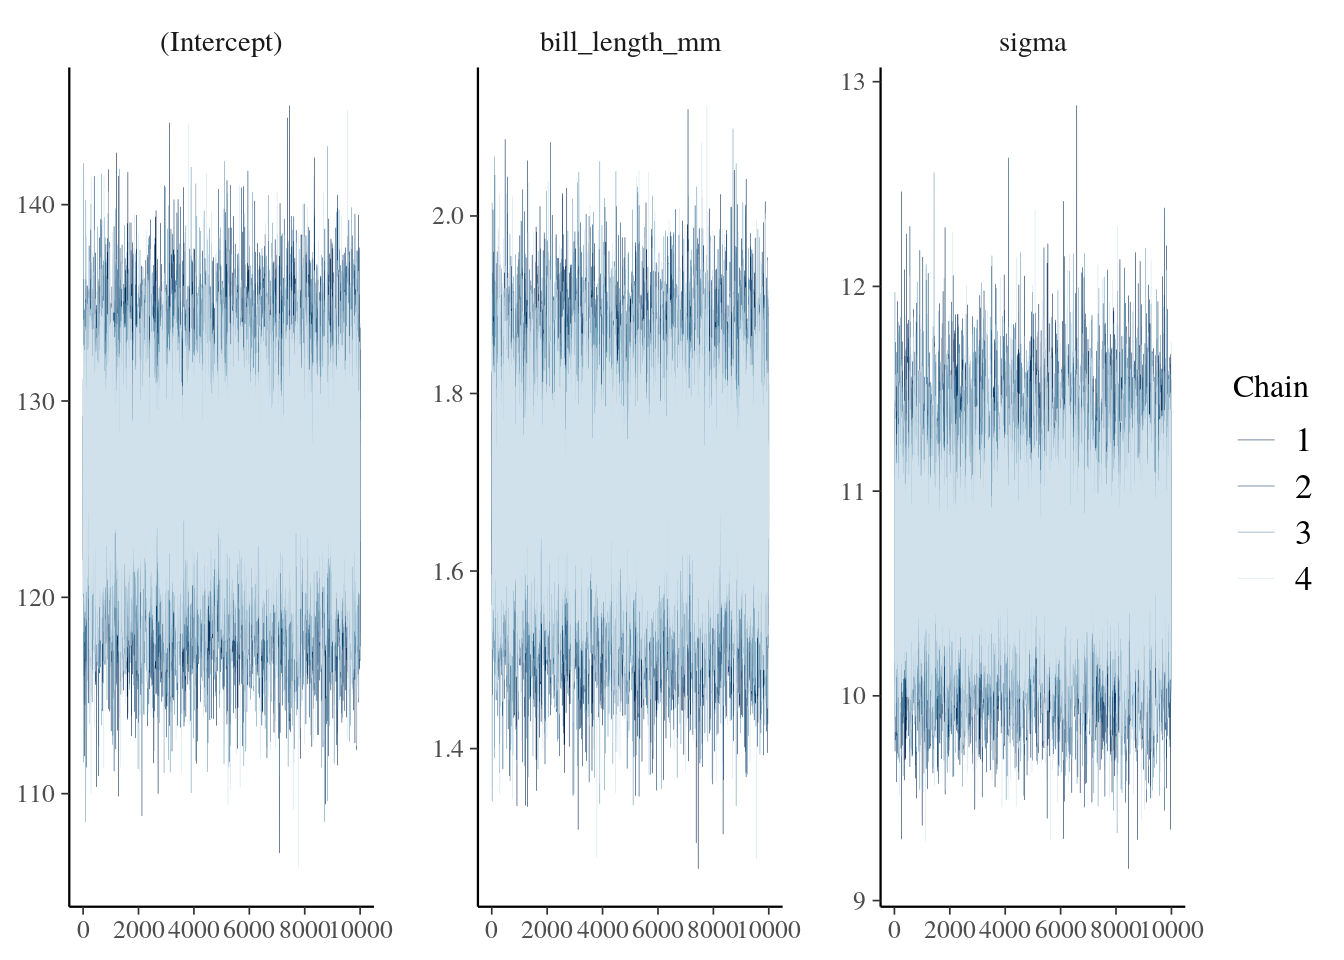
\includegraphics{ch9-10_files/figure-latex/unnamed-chunk-16-1.pdf}

\begin{enumerate}
\def\labelenumi{\alph{enumi}.}
\setcounter{enumi}{2}
\tightlist
\item
\end{enumerate}

\begin{Shaded}
\begin{Highlighting}[]
\FunctionTok{tidy}\NormalTok{(penguins\_post\_model, }\AttributeTok{conf.int =} \ConstantTok{TRUE}\NormalTok{, }\AttributeTok{conf.level =} \FloatTok{0.90}\NormalTok{)}
\end{Highlighting}
\end{Shaded}

\begin{verbatim}
## # A tibble: 2 x 5
##   term           estimate std.error conf.low conf.high
##   <chr>             <dbl>     <dbl>    <dbl>     <dbl>
## 1 (Intercept)      126.       4.67    118.      134.  
## 2 bill_length_mm     1.69     0.106     1.52      1.87
\end{verbatim}

\begin{enumerate}
\def\labelenumi{\alph{enumi}.}
\setcounter{enumi}{3}
\tightlist
\item
\end{enumerate}

There is a 90\% probability that the true bill\_length\_mm lies within
.1.5-.1.9.

\begin{enumerate}
\def\labelenumi{\alph{enumi}.}
\setcounter{enumi}{4}
\tightlist
\item
\end{enumerate}

There is a decent standard error, so I'm wary to say that we have enough
evidence that they are related.

\hypertarget{chapter-10}{%
\section{Chapter 10}\label{chapter-10}}

\hypertarget{section-7}{%
\subsection{10.7}\label{section-7}}

\begin{enumerate}
\def\labelenumi{\alph{enumi}.}
\tightlist
\item
\end{enumerate}

\begin{Shaded}
\begin{Highlighting}[]
\NormalTok{problem7\_data }\OtherTok{\textless{}{-}} 
  \FunctionTok{tibble}\NormalTok{(}
    \AttributeTok{x =} \FunctionTok{c}\NormalTok{(}\DecValTok{12}\NormalTok{,}\DecValTok{10}\NormalTok{,}\DecValTok{4}\NormalTok{,}\DecValTok{8}\NormalTok{,}\DecValTok{6}\NormalTok{), }
    \AttributeTok{y =} \FunctionTok{c}\NormalTok{(}\DecValTok{20}\NormalTok{,}\DecValTok{17}\NormalTok{,}\DecValTok{4}\NormalTok{,}\DecValTok{11}\NormalTok{,}\DecValTok{9}\NormalTok{)}
\NormalTok{  )}
\end{Highlighting}
\end{Shaded}

\$\$

y=mx+b \textbackslash{}

y= \beta\_1x+\beta\_0 \textbackslash{}

y= \beta\_0 + \beta\_1x \textbackslash{}

\hat{y}\_i= \beta\_0 + \beta\_1 x\_i \textbackslash{}

\hat{y}\_1= -1.8 + 2.1 \cdot 12 \textbackslash{}

\hat{y}\_2= -1.8 + 2.1 \cdot 10 \textbackslash{}

\$\$

\begin{enumerate}
\def\labelenumi{\alph{enumi}.}
\setcounter{enumi}{1}
\tightlist
\item
\end{enumerate}

\begin{Shaded}
\begin{Highlighting}[]
\NormalTok{problem7\_data }\SpecialCharTok{|\textgreater{}}
  \FunctionTok{mutate}\NormalTok{(}\AttributeTok{y\_hat=}\SpecialCharTok{{-}}\FloatTok{1.8+2.1}\SpecialCharTok{*}\NormalTok{x, }
         \AttributeTok{y\_model=}\SpecialCharTok{{-}}\FloatTok{1.8+2.1}\SpecialCharTok{*}\NormalTok{x}\SpecialCharTok{+}\FunctionTok{rnorm}\NormalTok{(}\DecValTok{5}\NormalTok{,}\DecValTok{0}\NormalTok{,}\FloatTok{0.8}\NormalTok{),}
         \AttributeTok{y\_model2=}\FunctionTok{rnorm}\NormalTok{(}\DecValTok{5}\NormalTok{,}\SpecialCharTok{{-}}\FloatTok{1.8+2.1}\SpecialCharTok{*}\NormalTok{x,}\FloatTok{0.8}\NormalTok{)}
\NormalTok{        )}
\end{Highlighting}
\end{Shaded}

\begin{verbatim}
## # A tibble: 5 x 5
##       x     y y_hat y_model y_model2
##   <dbl> <dbl> <dbl>   <dbl>    <dbl>
## 1    12    20  23.4   23.8     22.6 
## 2    10    17  19.2   18.5     20.9 
## 3     4     4   6.6    7.11     7.77
## 4     8    11  15     15.5     15.2 
## 5     6     9  10.8   10.9     10.2
\end{verbatim}

\hypertarget{section-8}{%
\subsection{10.13}\label{section-8}}

\begin{enumerate}
\def\labelenumi{\alph{enumi}.}
\tightlist
\item
\end{enumerate}

\begin{Shaded}
\begin{Highlighting}[]
\FunctionTok{head}\NormalTok{(coffee\_ratings)}
\end{Highlighting}
\end{Shaded}

\begin{verbatim}
## # A tibble: 6 x 27
##   owner       farm_name mill  in_country_part~ country_of_orig~ altitude_low_me~
##   <fct>       <fct>     <fct> <fct>            <fct>                       <dbl>
## 1 metad plc   "metad p~ meta~ METAD Agricultu~ Ethiopia                     1950
## 2 metad plc   "metad p~ meta~ METAD Agricultu~ Ethiopia                     1950
## 3 grounds fo~ "san mar~ <NA>  Specialty Coffe~ Guatemala                    1600
## 4 yidnekache~ "yidneka~ wole~ METAD Agricultu~ Ethiopia                     1800
## 5 metad plc   "metad p~ meta~ METAD Agricultu~ Ethiopia                     1950
## 6 ji-ae ahn    <NA>     <NA>  Specialty Coffe~ Brazil                         NA
## # ... with 21 more variables: altitude_high_meters <dbl>,
## #   altitude_mean_meters <dbl>, number_of_bags <dbl>, bag_weight <fct>,
## #   species <fct>, variety <fct>, processing_method <fct>, aroma <dbl>,
## #   flavor <dbl>, aftertaste <dbl>, acidity <dbl>, body <dbl>, balance <dbl>,
## #   uniformity <dbl>, clean_cup <dbl>, sweetness <dbl>, moisture <dbl>,
## #   category_one_defects <dbl>, category_two_defects <dbl>, color <fct>,
## #   total_cup_points <dbl>
\end{verbatim}

It likely violates the independence assumption due to aroma and
aftertaste not being completely independent. Also, other variables come
into play, such as sweetness, clean\_cup, and acidity.

\begin{enumerate}
\def\labelenumi{\alph{enumi}.}
\setcounter{enumi}{1}
\tightlist
\item
\end{enumerate}

\begin{Shaded}
\begin{Highlighting}[]
\FunctionTok{set.seed}\NormalTok{(}\DecValTok{84735}\NormalTok{)}
\NormalTok{new\_coffee }\OtherTok{\textless{}{-}}\NormalTok{ coffee\_ratings }\SpecialCharTok{\%\textgreater{}\%} 
  \FunctionTok{group\_by}\NormalTok{(farm\_name) }\SpecialCharTok{\%\textgreater{}\%} 
  \FunctionTok{sample\_n}\NormalTok{(}\DecValTok{1}\NormalTok{) }\SpecialCharTok{\%\textgreater{}\%} 
  \FunctionTok{ungroup}\NormalTok{()}
\FunctionTok{dim}\NormalTok{(new\_coffee)}
\end{Highlighting}
\end{Shaded}

\begin{verbatim}
## [1] 572  27
\end{verbatim}

\hypertarget{section-9}{%
\subsection{10.14}\label{section-9}}

\begin{enumerate}
\def\labelenumi{\alph{enumi}.}
\tightlist
\item
\end{enumerate}

\begin{Shaded}
\begin{Highlighting}[]
\FunctionTok{ggplot}\NormalTok{(new\_coffee, }\FunctionTok{aes}\NormalTok{(}\AttributeTok{x =}\NormalTok{ aroma, }\AttributeTok{y =}\NormalTok{ total\_cup\_points)) }\SpecialCharTok{+} 
  \FunctionTok{geom\_point}\NormalTok{(}\AttributeTok{size =} \FloatTok{0.5}\NormalTok{) }\SpecialCharTok{+} 
  \FunctionTok{geom\_smooth}\NormalTok{(}\AttributeTok{method =} \StringTok{"lm"}\NormalTok{, }\AttributeTok{se =} \ConstantTok{FALSE}\NormalTok{)}
\end{Highlighting}
\end{Shaded}

\begin{verbatim}
## `geom_smooth()` using formula 'y ~ x'
\end{verbatim}

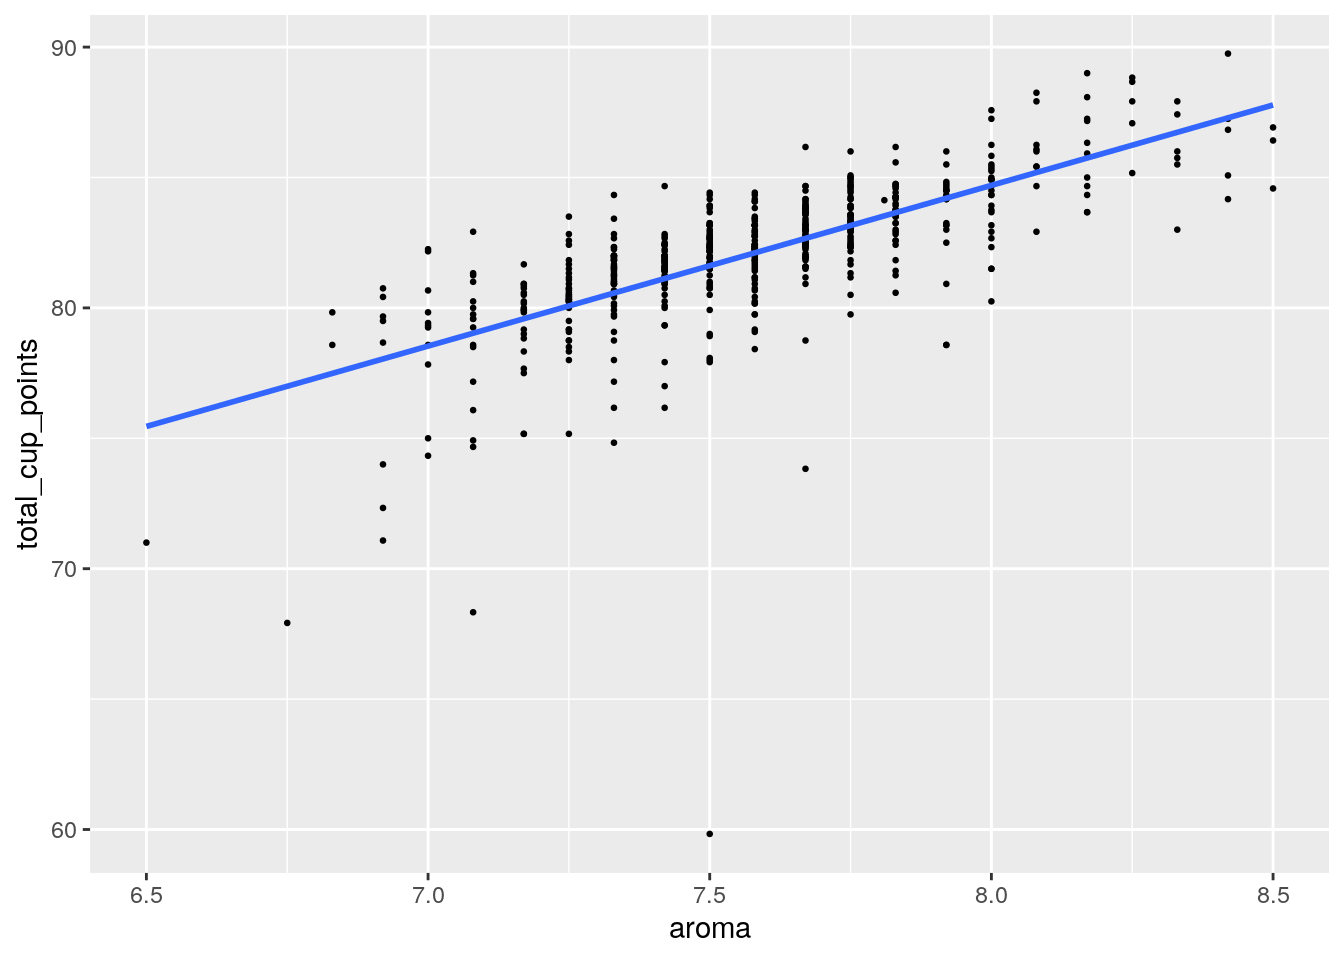
\includegraphics{ch9-10_files/figure-latex/unnamed-chunk-21-1.pdf}

\begin{enumerate}
\def\labelenumi{\alph{enumi}.}
\setcounter{enumi}{1}
\tightlist
\item
\end{enumerate}

\begin{Shaded}
\begin{Highlighting}[]
\FunctionTok{summary}\NormalTok{(new\_coffee)}
\end{Highlighting}
\end{Shaded}

\begin{verbatim}
##                             owner            farm_name  
##  cqi taiwan icp cqi台灣合作夥伴: 44   -           :  1  
##  juan luis alvarado romero     : 40   1           :  1  
##  nucoffee                      : 26   200 farms   :  1  
##  lin, che-hao krude 林哲豪     : 20   2000 farmers:  1  
##  alfredo bojalil               : 14   2000 farms  :  1  
##  (Other)                       :425   (Other)     :566  
##  NA's                          :  3   NA's        :  1  
##                                mill    
##  beneficio ixchel                : 16  
##  beneficio exportacafe agua santa:  9  
##  mzuzu coffee coop union         :  9  
##  zaragoza itundujia, oaxaca      :  9  
##  agroindustrias unidas de mexico :  8  
##  (Other)                         :435  
##  NA's                            : 86  
##                            in_country_partner
##  AMECAFE                            :156     
##  Specialty Coffee Association       : 95     
##  Blossom Valley International       : 52     
##  Africa Fine Coffee Association     : 41     
##  Asociacion Nacional Del Café       : 40     
##  Uganda Coffee Development Authority: 30     
##  (Other)                            :158     
##                     country_of_origin altitude_low_meters altitude_high_meters
##  Mexico                      :170     Min.   :   12       Min.   :   12       
##  Taiwan                      : 64     1st Qu.: 1015       1st Qu.: 1094       
##  Brazil                      : 51     Median : 1250       Median : 1300       
##  Guatemala                   : 50     Mean   : 1283       Mean   : 1327       
##  Tanzania, United Republic Of: 34     3rd Qu.: 1500       3rd Qu.: 1569       
##  Uganda                      : 29     Max.   :11000       Max.   :11000       
##  (Other)                     :174     NA's   :36          NA's   :36          
##  altitude_mean_meters number_of_bags     bag_weight     species   
##  Min.   :   12        Min.   :   1.0   1 kg   :199   Arabica:558  
##  1st Qu.: 1050        1st Qu.:  10.0   60 kg  :158   Robusta: 14  
##  Median : 1270        Median :  38.5   69 kg  : 59                
##  Mean   : 1305        Mean   : 108.6   2 kg   : 53                
##  3rd Qu.: 1550        3rd Qu.: 250.0   30 kg  : 24                
##  Max.   :11000        Max.   :1062.0   20 kg  : 10                
##  NA's   :36                            (Other): 69                
##     variety                    processing_method     aroma      
##  Typica :166   Natural / Dry            : 94     Min.   :6.500  
##  Bourbon: 83   Other                    : 16     1st Qu.:7.330  
##  Other  : 66   Pulped natural / honey   :  5     Median :7.580  
##  Caturra: 55   Semi-washed / Semi-pulped: 41     Mean   :7.578  
##  Catuai : 36   Washed / Wet             :365     3rd Qu.:7.750  
##  (Other):109   NA's                     : 51     Max.   :8.500  
##  NA's   : 57                                                    
##      flavor        aftertaste       acidity           body      
##  Min.   :6.080   Min.   :6.170   Min.   :6.080   Min.   :5.170  
##  1st Qu.:7.330   1st Qu.:7.170   1st Qu.:7.330   1st Qu.:7.330  
##  Median :7.500   Median :7.420   Median :7.500   Median :7.500  
##  Mean   :7.527   Mean   :7.395   Mean   :7.533   Mean   :7.502  
##  3rd Qu.:7.750   3rd Qu.:7.580   3rd Qu.:7.750   3rd Qu.:7.670  
##  Max.   :8.670   Max.   :8.580   Max.   :8.500   Max.   :8.500  
##                                                                 
##     balance        uniformity       clean_cup        sweetness     
##  Min.   :5.250   Min.   : 6.670   Min.   : 0.000   Min.   : 1.330  
##  1st Qu.:7.250   1st Qu.:10.000   1st Qu.:10.000   1st Qu.:10.000  
##  Median :7.500   Median :10.000   Median :10.000   Median :10.000  
##  Mean   :7.479   Mean   : 9.887   Mean   : 9.823   Mean   : 9.882  
##  3rd Qu.:7.670   3rd Qu.:10.000   3rd Qu.:10.000   3rd Qu.:10.000  
##  Max.   :8.580   Max.   :10.000   Max.   :10.000   Max.   :10.000  
##                                                                    
##     moisture       category_one_defects category_two_defects          color    
##  Min.   :0.00000   Min.   : 0.0000      Min.   : 0.000       Blue-Green  : 44  
##  1st Qu.:0.10000   1st Qu.: 0.0000      1st Qu.: 0.000       Bluish-Green: 43  
##  Median :0.11000   Median : 0.0000      Median : 2.000       Green       :371  
##  Mean   :0.09846   Mean   : 0.4161      Mean   : 3.932       None        : 37  
##  3rd Qu.:0.12000   3rd Qu.: 0.0000      3rd Qu.: 5.000       NA's        : 77  
##  Max.   :0.20000   Max.   :31.0000      Max.   :47.000                         
##                                                                                
##  total_cup_points
##  Min.   :59.83   
##  1st Qu.:80.92   
##  Median :82.33   
##  Mean   :82.10   
##  3rd Qu.:83.58   
##  Max.   :89.75   
## 
\end{verbatim}

\begin{Shaded}
\begin{Highlighting}[]
\NormalTok{coffee\_model }\OtherTok{\textless{}{-}} \FunctionTok{stan\_glm}\NormalTok{(total\_cup\_points }\SpecialCharTok{\textasciitilde{}}\NormalTok{ aroma, }\AttributeTok{data =}\NormalTok{ new\_coffee,}
                       \AttributeTok{family =}\NormalTok{ gaussian,}
                       \AttributeTok{prior\_intercept =} \FunctionTok{normal}\NormalTok{(}\FloatTok{7.5}\NormalTok{, }\FloatTok{1.2}\NormalTok{),}
                       \AttributeTok{prior =} \FunctionTok{normal}\NormalTok{(}\FloatTok{82.10}\NormalTok{, }\DecValTok{30}\NormalTok{), }
                       \AttributeTok{prior\_aux =} \FunctionTok{exponential}\NormalTok{(}\FloatTok{0.0008}\NormalTok{),}
                       \AttributeTok{chains =} \DecValTok{4}\NormalTok{, }\AttributeTok{iter =} \DecValTok{10000}\SpecialCharTok{*}\DecValTok{2}\NormalTok{, }\AttributeTok{seed =} \DecValTok{84735}\NormalTok{)}
\end{Highlighting}
\end{Shaded}

\begin{verbatim}
## 
## SAMPLING FOR MODEL 'continuous' NOW (CHAIN 1).
## Chain 1: 
## Chain 1: Gradient evaluation took 2.2e-05 seconds
## Chain 1: 1000 transitions using 10 leapfrog steps per transition would take 0.22 seconds.
## Chain 1: Adjust your expectations accordingly!
## Chain 1: 
## Chain 1: 
## Chain 1: Iteration:     1 / 20000 [  0%]  (Warmup)
## Chain 1: Iteration:  2000 / 20000 [ 10%]  (Warmup)
## Chain 1: Iteration:  4000 / 20000 [ 20%]  (Warmup)
## Chain 1: Iteration:  6000 / 20000 [ 30%]  (Warmup)
## Chain 1: Iteration:  8000 / 20000 [ 40%]  (Warmup)
## Chain 1: Iteration: 10000 / 20000 [ 50%]  (Warmup)
## Chain 1: Iteration: 10001 / 20000 [ 50%]  (Sampling)
## Chain 1: Iteration: 12000 / 20000 [ 60%]  (Sampling)
## Chain 1: Iteration: 14000 / 20000 [ 70%]  (Sampling)
## Chain 1: Iteration: 16000 / 20000 [ 80%]  (Sampling)
## Chain 1: Iteration: 18000 / 20000 [ 90%]  (Sampling)
## Chain 1: Iteration: 20000 / 20000 [100%]  (Sampling)
## Chain 1: 
## Chain 1:  Elapsed Time: 0.251166 seconds (Warm-up)
## Chain 1:                0.779766 seconds (Sampling)
## Chain 1:                1.03093 seconds (Total)
## Chain 1: 
## 
## SAMPLING FOR MODEL 'continuous' NOW (CHAIN 2).
## Chain 2: 
## Chain 2: Gradient evaluation took 9e-06 seconds
## Chain 2: 1000 transitions using 10 leapfrog steps per transition would take 0.09 seconds.
## Chain 2: Adjust your expectations accordingly!
## Chain 2: 
## Chain 2: 
## Chain 2: Iteration:     1 / 20000 [  0%]  (Warmup)
## Chain 2: Iteration:  2000 / 20000 [ 10%]  (Warmup)
## Chain 2: Iteration:  4000 / 20000 [ 20%]  (Warmup)
## Chain 2: Iteration:  6000 / 20000 [ 30%]  (Warmup)
## Chain 2: Iteration:  8000 / 20000 [ 40%]  (Warmup)
## Chain 2: Iteration: 10000 / 20000 [ 50%]  (Warmup)
## Chain 2: Iteration: 10001 / 20000 [ 50%]  (Sampling)
## Chain 2: Iteration: 12000 / 20000 [ 60%]  (Sampling)
## Chain 2: Iteration: 14000 / 20000 [ 70%]  (Sampling)
## Chain 2: Iteration: 16000 / 20000 [ 80%]  (Sampling)
## Chain 2: Iteration: 18000 / 20000 [ 90%]  (Sampling)
## Chain 2: Iteration: 20000 / 20000 [100%]  (Sampling)
## Chain 2: 
## Chain 2:  Elapsed Time: 0.246289 seconds (Warm-up)
## Chain 2:                0.843513 seconds (Sampling)
## Chain 2:                1.0898 seconds (Total)
## Chain 2: 
## 
## SAMPLING FOR MODEL 'continuous' NOW (CHAIN 3).
## Chain 3: 
## Chain 3: Gradient evaluation took 8e-06 seconds
## Chain 3: 1000 transitions using 10 leapfrog steps per transition would take 0.08 seconds.
## Chain 3: Adjust your expectations accordingly!
## Chain 3: 
## Chain 3: 
## Chain 3: Iteration:     1 / 20000 [  0%]  (Warmup)
## Chain 3: Iteration:  2000 / 20000 [ 10%]  (Warmup)
## Chain 3: Iteration:  4000 / 20000 [ 20%]  (Warmup)
## Chain 3: Iteration:  6000 / 20000 [ 30%]  (Warmup)
## Chain 3: Iteration:  8000 / 20000 [ 40%]  (Warmup)
## Chain 3: Iteration: 10000 / 20000 [ 50%]  (Warmup)
## Chain 3: Iteration: 10001 / 20000 [ 50%]  (Sampling)
## Chain 3: Iteration: 12000 / 20000 [ 60%]  (Sampling)
## Chain 3: Iteration: 14000 / 20000 [ 70%]  (Sampling)
## Chain 3: Iteration: 16000 / 20000 [ 80%]  (Sampling)
## Chain 3: Iteration: 18000 / 20000 [ 90%]  (Sampling)
## Chain 3: Iteration: 20000 / 20000 [100%]  (Sampling)
## Chain 3: 
## Chain 3:  Elapsed Time: 0.244978 seconds (Warm-up)
## Chain 3:                0.864368 seconds (Sampling)
## Chain 3:                1.10935 seconds (Total)
## Chain 3: 
## 
## SAMPLING FOR MODEL 'continuous' NOW (CHAIN 4).
## Chain 4: 
## Chain 4: Gradient evaluation took 9e-06 seconds
## Chain 4: 1000 transitions using 10 leapfrog steps per transition would take 0.09 seconds.
## Chain 4: Adjust your expectations accordingly!
## Chain 4: 
## Chain 4: 
## Chain 4: Iteration:     1 / 20000 [  0%]  (Warmup)
## Chain 4: Iteration:  2000 / 20000 [ 10%]  (Warmup)
## Chain 4: Iteration:  4000 / 20000 [ 20%]  (Warmup)
## Chain 4: Iteration:  6000 / 20000 [ 30%]  (Warmup)
## Chain 4: Iteration:  8000 / 20000 [ 40%]  (Warmup)
## Chain 4: Iteration: 10000 / 20000 [ 50%]  (Warmup)
## Chain 4: Iteration: 10001 / 20000 [ 50%]  (Sampling)
## Chain 4: Iteration: 12000 / 20000 [ 60%]  (Sampling)
## Chain 4: Iteration: 14000 / 20000 [ 70%]  (Sampling)
## Chain 4: Iteration: 16000 / 20000 [ 80%]  (Sampling)
## Chain 4: Iteration: 18000 / 20000 [ 90%]  (Sampling)
## Chain 4: Iteration: 20000 / 20000 [100%]  (Sampling)
## Chain 4: 
## Chain 4:  Elapsed Time: 0.252697 seconds (Warm-up)
## Chain 4:                0.839688 seconds (Sampling)
## Chain 4:                1.09238 seconds (Total)
## Chain 4:
\end{verbatim}

\begin{enumerate}
\def\labelenumi{\alph{enumi}.}
\setcounter{enumi}{2}
\tightlist
\item
\end{enumerate}

\begin{Shaded}
\begin{Highlighting}[]
\FunctionTok{mcmc\_trace}\NormalTok{(coffee\_model, }\AttributeTok{size =} \FloatTok{0.1}\NormalTok{)}
\end{Highlighting}
\end{Shaded}

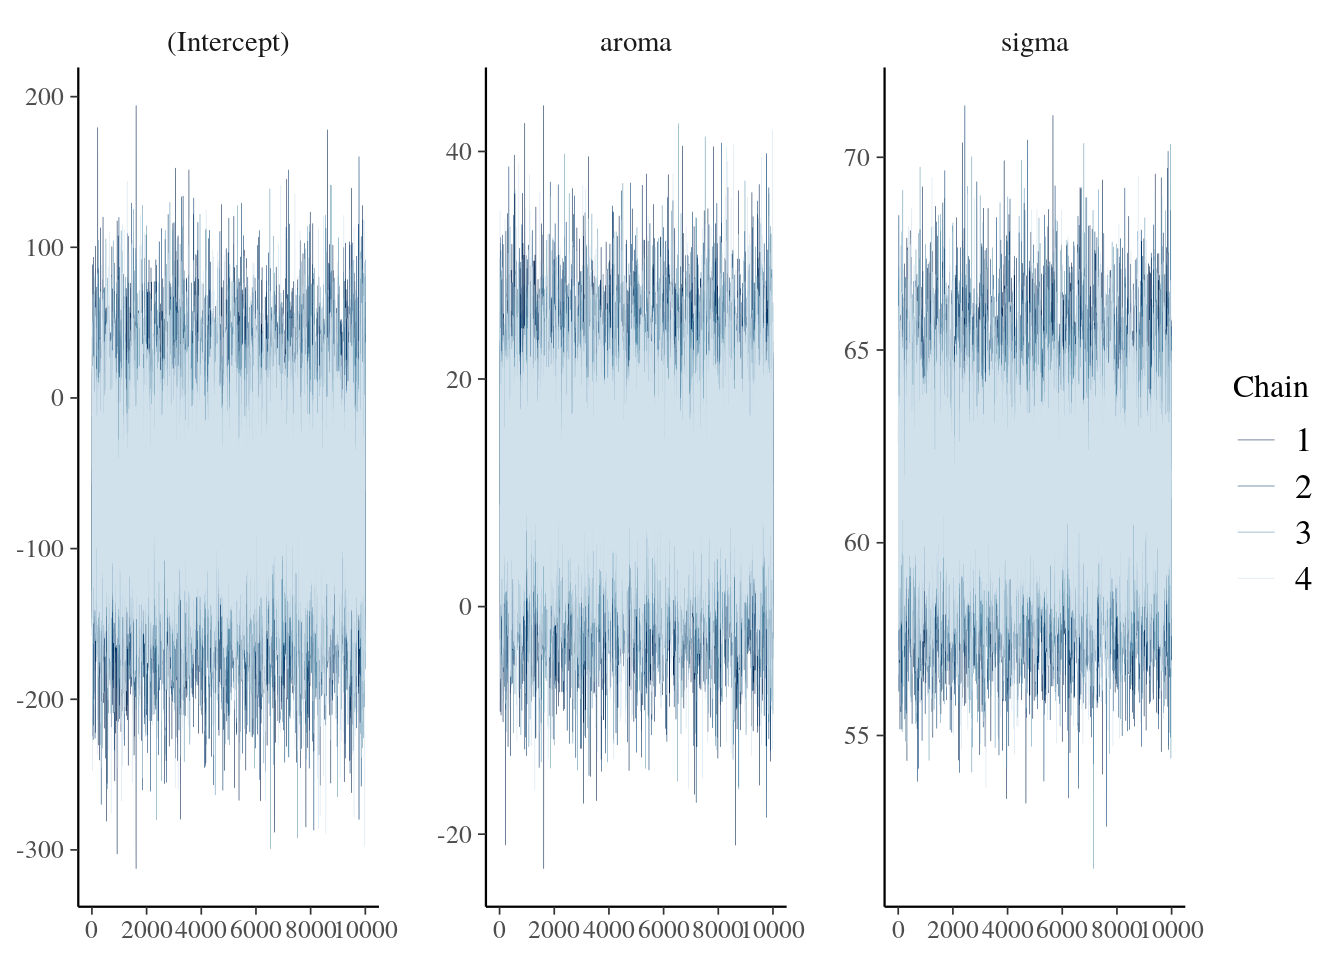
\includegraphics{ch9-10_files/figure-latex/unnamed-chunk-24-1.pdf}

\begin{enumerate}
\def\labelenumi{\alph{enumi}.}
\setcounter{enumi}{3}
\tightlist
\item
\end{enumerate}

\begin{Shaded}
\begin{Highlighting}[]
\FunctionTok{summary}\NormalTok{(coffee\_model)}
\end{Highlighting}
\end{Shaded}

\begin{verbatim}
## 
## Model Info:
##  function:     stan_glm
##  family:       gaussian [identity]
##  formula:      total_cup_points ~ aroma
##  algorithm:    sampling
##  sample:       40000 (posterior sample size)
##  priors:       see help('prior_summary')
##  observations: 572
##  predictors:   2
## 
## Estimates:
##               mean   sd     10%    50%    90% 
## (Intercept)  -65.6   60.2 -143.3  -65.3   11.5
## aroma         11.4    7.9    1.3   11.4   21.7
## sigma         61.4    2.3   58.5   61.4   64.3
## 
## Fit Diagnostics:
##            mean   sd   10%   50%   90%
## mean_PPD 20.9    2.9 17.2  21.0  24.6 
## 
## The mean_ppd is the sample average posterior predictive distribution of the outcome variable (for details see help('summary.stanreg')).
## 
## MCMC diagnostics
##               mcse Rhat n_eff
## (Intercept)   0.3  1.0  30160
## aroma         0.0  1.0  30212
## sigma         0.0  1.0  21874
## mean_PPD      0.0  1.0  33412
## log-posterior 0.0  1.0  16598
## 
## For each parameter, mcse is Monte Carlo standard error, n_eff is a crude measure of effective sample size, and Rhat is the potential scale reduction factor on split chains (at convergence Rhat=1).
\end{verbatim}

\begin{enumerate}
\def\labelenumi{\alph{enumi}.}
\setcounter{enumi}{4}
\tightlist
\item
\end{enumerate}

Aroma and rating are associated. The better a coffee's aroma is, the
rating is likely to be better as well.

\hypertarget{section-10}{%
\subsection{10.15}\label{section-10}}

\begin{enumerate}
\def\labelenumi{\alph{enumi}.}
\tightlist
\item
\item
\item
\item
\end{enumerate}

\hypertarget{section-11}{%
\subsection{10.16}\label{section-11}}

\begin{enumerate}
\def\labelenumi{\alph{enumi}.}
\tightlist
\item
\item
\item
\item
\end{enumerate}

\hypertarget{section-12}{%
\subsection{10.17}\label{section-12}}

\begin{enumerate}
\def\labelenumi{\alph{enumi}.}
\tightlist
\item
\item
\item
\end{enumerate}

\hypertarget{section-13}{%
\subsection{10.18}\label{section-13}}

\hypertarget{section-14}{%
\subsection{10.19}\label{section-14}}

\begin{enumerate}
\def\labelenumi{\alph{enumi}.}
\tightlist
\item
\item
\item
\item
\end{enumerate}

\end{document}
